\begin{dang}{Tương giao khi đề cho bảng biến thiên hoặc đồ thị}
    \baitoan Cho hàm số có bảng biến thiên hoặc đồ thị hàm số. Các yêu cầu thường gặp bao gồm:
    \begin{itemize}
        \item Biện luận số nghiệm của phương trình không chứa tham số.
        \item Tìm điều kiện của tham số thỏa mãn điều kiện liên quan tới nghiệm của phương trình.
    \end{itemize}
    \phuongphap
    \begin{enumerate}
        \item[] {\bf Bước 1:} Biến đổi phương trình bài toán đưa ra về dạng liên quan với hàm số được cho bảng biến thiên hoặc đồ thị ở đầu bài.
        \item[] {\bf Bước 2:} Biện luận kết quả bài toán dựa trên đồ thị hoặc bảng biến thiên đưa ra ở đề bài.
    \end{enumerate}
    \begin{luuy}
        \begin{itemize}
            \item Số nghiệm của phương trình $f(x)=m$ là số giao điểm của đường thẳng $y=m$ với đồ thị của hàm số $y=f(x)$.
            \item Số nghiệm của phương trình $f(x)=g(x)$ là số giao điểm của hai đồ thị của các hàm số $y=f(x)$ và $y=g(x)$.
        \end{itemize}
    \end{luuy}
\end{dang}
\begin{vd}%[2D1B5-4]
    Cho hàm số $f(x) = ax^3 +bx^2 +cx+d$ có đồ thị như hình bên.
    \immini{\begin{enumEX}[1.]{1}
            \item Phương trình $f(x)+2 =0$ có tất cả bao nhiêu nghiệm dương?
            \item Phương trình $3f(x)+2=0$ có tất cả bao nhiêu nghiệm âm?
            \item Phương trình $f(x)-2=0$ có tất cả bao nhiêu nghiệm dương? \item Phương trình $2f(x)-1=0$ có tất cả bao nhiêu nghiệm nhỏ hơn 1?
            \item Phương trình $2f(x)-3=0$ có tất cả bao nhiêu nghiệm nhỏ hơn 2?
            \item Phương trình $2f(x)-5=0$ có tất cả bao nhiêu nghiệm lớn hơn $-1$?
        \end{enumEX}
    }{\begin{tikzpicture}[scale=.8, font=\footnotesize, line join=round, line cap=round, >=stealth]
            \def\xmin{-3}\def\xmax{3}\def\ymin{-2}\def\ymax{4}
            \draw[->] (\xmin-0.2,0)--(\xmax+0.2,0) node[below] {\footnotesize $x$};
            \draw[->] (0,\ymin-0.2)--(0,\ymax+0.2) node[right] {\footnotesize $y$};
            \draw (0,0) node [below left] {\footnotesize $O$};
            \foreach \x in {-1,2}\draw (\x,0.1)--(\x,-0.1) node [below] {\footnotesize $\x$};
            \foreach \x in {1}\draw (\x,-0.1)--(\x,0.1) node [above] {\footnotesize $\x$};
            \foreach \x in {-2}\draw (\x,-0.1)--(\x,0.1) node [above left] {\footnotesize $\x$};
            \foreach \y in {-1,1}\draw (0.1,\y)--(-0.1,\y) node [left] {\footnotesize $\y$};
            \foreach \y in {3}\draw (0.1,\y)--(-0.1,\y) node [above left] {\footnotesize $\y$};
            \clip (\xmin,\ymin) rectangle (\xmax,\ymax);
            \draw[smooth,samples=200,domain=\xmin:\xmax] plot (\x,{1*((\x)^3)+0*((\x)^2)+-3*(\x)+1});
            \draw[dashed] (0.0,0)--(0.0,1.0)--(0,1.0);\fill (0.0,1.0) circle (1pt);
            \draw[dashed] (-1.0,0)--(-1.0,3.0)--(0,3.0);
            \draw[dashed] (1.0,0)--(1.0,-1.0)--(0,-1.0);
            \draw[dashed] (2,0)--(2,3)--(0,3);
    \end{tikzpicture}}
    \loigiai{}
\end{vd}
%\loigiai{
% \begin{enumEX}[1.]{1}
% \item $f(x)+2 =0\Leftrightarrow f(x)=-2$.\\ Số nghiệm của phương trình là số giao điểm của $(C) \colon y=f(x)$ (hình vẽ) và $d \colon y=-2.$\\Vậy phương trình không có nghiệm dương.
% \item $3f(x)+2=0\Leftrightarrow f(x)=-\dfrac{2}{3}$.\\ Số nghiệm của phương trình là số giao điểm của $(C) \colon y=f(x)$ (hình vẽ) và $d \colon y=-\dfrac{2}{3}.$\\Vậy phương trình có 1 nghiệm âm.
% \item $f(x)-2=0\Leftrightarrow f(x)=2$.\\ Số nghiệm của phương trình là số giao điểm của $(C) \colon y=f(x)$ (hình vẽ) và $d \colon y=2.$\\Vậy phương trình có 1 nghiệm dương.
% \item $2f(x)-1=0\Leftrightarrow f(x)=\dfrac{1}{2}$.\\ Số nghiệm của phương trình là số giao điểm của $(C) \colon y=f(x)$ (hình vẽ) và $d \colon y=\dfrac{1}{2}.$\\Vậy phương trình có 2 nghiệm nhỏ hơn 1.
% \item $2f(x)-3=0\Leftrightarrow f(x)=\dfrac{3}{2}$.\\ Số nghiệm của phương trình là số giao điểm của $(C) \colon y=f(x)$ (hình vẽ) và $d \colon y=\dfrac{3}{2}.$\\Vậy phương trình có 3 nghiệm nhỏ hơn 2?
% \item $2f(x)-5=0\Leftrightarrow f(x)=\dfrac{5}{2}$.\\ Số nghiệm của phương trình là số giao điểm của $(C) \colon y=f(x)$ (hình vẽ) và $d \colon y=\dfrac{5}{2}.$\\Vậy phương trình có 2 nghiệm lớn hơn $-1$?
% \end{enumEX}
%
%}
\begin{vd}%[2D1B5-4]
    Cho hàm số $f(x)=ax^3+bx^2+cx+d$ có đồ thị là hình bên dưới
    \immini{\begin{enumEX}[1.]{1}
            \item Tìm $m$ để phương trình $f(x)=m$ có đúng một nghiệm.
            \item Tìm $m$ để phương trình $f(x)=2m-1$ có đúng hai nghiệm.
            \item Tìm $m$ để phương trình $f(x)-1=m$ có đúng ba nghiệm.
            \item Tìm $m$ để phương trình $f(x)=m$ có đúng một nghiệm dương.
            \item Tìm $m$ để phương trình $f(x)=m$ có đúng một nghiệm âm
    \end{enumEX}}{\begin{tikzpicture}[scale=.7, font=\footnotesize, >=stealth]
            \def\xmin{-3}\def\xmax{3}\def\ymin{-2}\def\ymax{5}
            \draw[->] (\xmin-0.2,0)--(\xmax+0.2,0) node[below] {\footnotesize $x$};
            \draw[->] (0,\ymin-0.2)--(0,\ymax+0.2) node[right] {\footnotesize $y$};
            \draw($(0,0)$)node[below left]{$O$};
            \draw($(-1,0)$)node[below]{$-1$};
            \draw($(2,0)$)node[above right]{$2$};
            \draw($(0,2)$)node[left]{$2$};
            \draw[dashed] (-2,0)node[below]{$-2$}|-(0,4)node[above left]{$4$};
            \draw[dashed] (1,0)node[below]{$1$}|-(1,4)|-(0,4);
            \clip (\xmin,\ymin) rectangle (\xmax,\ymax);
            \draw[smooth,samples=200,domain=\xmin:\xmax] plot (\x,{-1*((\x)^3)+-0*((\x)^2)+3*(\x)+2});
    \end{tikzpicture}}
    % \loigiai{
    % \begin{enumEX}[1.]{1}
    % \item Số nghiệm của phương trình $f(x)=m$ chính là số giao điểm của $(C)\colon y=f(x)$ (hình vẽ) và đường thẳng $d\colon y=m$.\\
    % Phương trình $f(x)=m$ có đúng một nghiệm khi và chỉ khi $(C)\colon y=f(x)$ và đường thẳng $d\colon y=m$ có đúng một giao điểm
    % \[\Leftrightarrow\hoac{&m<0\\&m>4.}\]
    % Vậy $m\in (-\infty;0)\cup (4;+\infty)$ thì phương trình $f(x)=m$ có đúng một nghiệm.
    % \item Số nghiệm của phương trình $f(x)=2m-1$ chính là số giao điểm của $(C)\colon y=f(x)$ (hình vẽ) và đường thẳng $d\colon y=2m-1$.\\
    % Phương trình $f(x)=2m-1$ có đúng hai nghiệm khi và chỉ khi $(C)\colon y=f(x)$ và đường thẳng $d\colon y=2m-1$ có đúng hai giao điểm
    % \[\Leftrightarrow\hoac{&2m-1=0\\&2m-1=4}\Leftrightarrow \hoac{&m=\dfrac{1}{2}\\&m=\dfrac{5}{2}.}\]
    % Vậy $m\in\left\{\dfrac{1}{2};\dfrac{5}{2}\right\}$ thì phương trình $f(x)=m$ có đúng hai nghiệm.
    % \item Phương trình $f(x)-1=m\Leftrightarrow f(x)=m+1$.\\
    % Số nghiệm của phương trình $f(x)=m+1$ chính là số giao điểm của $(C)\colon y=f(x)$ (hình vẽ) và đường thẳng $d\colon y=m+1$.\\
    % Phương trình $f(x)=m+1$ có đúng ba nghiệm khi và chỉ khi $(C)\colon y=f(x)$ và đường thẳng $d\colon y=m+1$ có đúng ba giao điểm
    % \[\Leftrightarrow 0<m+1<4\Leftrightarrow -1<m<3.\]
    % Vậy $m\in (-1;3)$ thì phương trình $f(x)-1=m$ có đúng ba nghiệm.
    % \item Số nghiệm của phương trình $f(x)=m$ chính là số giao điểm của $(C)\colon y=f(x)$ (hình vẽ) và đường thẳng $d\colon y=m$.\\
    % Phương trình $f(x)=m$ có đúng một nghiệm dương khi và chỉ khi $(C)\colon y=f(x)$ và đường thẳng $d\colon y=m$ có đúng một giao điểm nằm phía bên phải trục tung
    % \[\Leftrightarrow m<0.\]
    % Vậy $ m<0$ thì phương trình $f(x)=m$ có đúng một nghiệm dương.
    % \item Số nghiệm của phương trình $f(x)=m$ chính là số giao điểm của $(C)\colon y=f(x)$ (hình vẽ) và đường thẳng $d\colon y=m$.\\
    % Phương trình $f(x)=m$ có đúng một nghiệm âm khi và chỉ khi $(C)\colon y=f(x)$ và đường thẳng $d\colon y=m$ có đúng một giao điểm nằm phía bên trái trục tung
    % \[\Leftrightarrow m>4.\]
    % Vậy $ m>4$ thì phương trình $f(x)=m$ có đúng một nghiệm âm.
    % \end{enumEX}}
    \loigiai{}
\end{vd}
\begin{vd}%[2D1B5-4]
    Cho hàm số $f(x) = ax^3 +bx^2 +cx+d$ có đồ thị như hình bên.
    \immini{
        \begin{enumEX}[1.]{1}
            \item Phương trình $f^2(x)-4f(x)+3=0$ có tất cả bao nhiêu nghiệm, trong đó có bao nhiêu nghiệm dương?
            \item Phương trình $f(x^2 - 3x +1)-3=0$ có tất cả bao nhiêu nghiệm?
            \item Phương trình $f(x)=x+1$ có tất cả bao nhiêu nghiệm?
            \item Phương trình $4f(x)= 3x^2$ có tất cả bao nhiêu nghiệm?
        \end{enumEX}
    }{\begin{tikzpicture}[scale=.8, font=\footnotesize, line join=round, line cap=round, >=stealth]
            \def\xmin{-3}\def\xmax{3}\def\ymin{-2}\def\ymax{4}
            \draw[->] (\xmin-0.2,0)--(\xmax+0.2,0) node[below] {\footnotesize $x$};
            \draw[->] (0,\ymin-0.2)--(0,\ymax+0.2) node[right] {\footnotesize $y$};
            \draw (0,0) node [below left] {\footnotesize $O$};
            \foreach \x in {-1,2}\draw (\x,0.1)--(\x,-0.1) node [below] {\footnotesize $\x$};
            \foreach \x in {1}\draw (\x,-0.1)--(\x,0.1) node [above] {\footnotesize $\x$};
            \foreach \x in {-2}\draw (\x,-0.1)--(\x,0.1) node [above left] {\footnotesize $\x$};
            \foreach \y in {-1,1}\draw (0.1,\y)--(-0.1,\y) node [left] {\footnotesize $\y$};
            \foreach \y in {3}\draw (0.1,\y)--(-0.1,\y) node [above left] {\footnotesize $\y$};
            \clip (\xmin,\ymin) rectangle (\xmax,\ymax);
            \draw[smooth,samples=200,domain=\xmin:\xmax] plot (\x,{1*((\x)^3)+0*((\x)^2)+-3*(\x)+1});
            \draw[dashed] (0.0,0)--(0.0,1.0)--(0,1.0);\fill (0.0,1.0) circle (1pt);
            \draw[dashed] (-1.0,0)--(-1.0,3.0)--(0,3.0);
            \draw[dashed] (1.0,0)--(1.0,-1.0)--(0,-1.0);
            \draw[dashed] (2,0)--(2,3)--(0,3);
    \end{tikzpicture}}
    \loigiai{}
\end{vd}
%\loigiai{
% \begin{enumEX}[1.]{1}
% \item Phương trình $f^2(x)-4f(x)+3=0\Leftrightarrow \hoac{&f(x)=1\\&f(x)=3.}$\\
% Tương tự ví dụ 1, ta có
% \begin{itemize}
% \item $f(x)=1$ có 3 nghiệm phân biệt, trong đó có 1 nghiệm dương.
% \item $f(x)=3$ có 2 nghiệm phân biệt, trong đó có 1 nghiệm dương.
% \end{itemize}
% Vậy phương trình $f^2(x)-4f(x)+3=0$ có tất cả 5 nghiệm, trong đó có 2 nghiệm dương.
%
% \item Phương trình $f(x^2 - 3x +1)-3=0\Leftrightarrow f(x^2 - 3x +1)=3$\\
% Tương tự ví dụ 1, ta có $f(x^2 - 3x +1)=3 \Leftrightarrow \hoac{&x^2 - 3x +1=-1&{\text{có 2 nghiệm} }\\&x^2 - 3x +1=2&{\text{có 2 nghiệm} }.}$\\
% Vậy phương trình $f(x^2 - 3x +1)-3=0$ có tất cả 4 nghiệm.
% \immini{\item Dựng đường thẳng $y=x+1$, ta có số nghiệm của phương trình $f(x)=x+1$ là số giao điểm của $(C) \colon y=f(x)$ và $d \colon y=x+1$ (hình vẽ). \\Vậy phương trình $f(x)=x+1$ có tất cả 3 nghiệm. }{\begin{tikzpicture}[scale=.8, font=\footnotesize, line join=round, line cap=round, >=stealth]
% \def\xmin{-3}\def\xmax{3}\def\ymin{-2}\def\ymax{4}
% \draw[->] (\xmin-0.2,0)--(\xmax+0.2,0) node[below] {\footnotesize $x$};
% \draw[->] (0,\ymin-0.2)--(0,\ymax+0.2) node[right] {\footnotesize $y$};
% \draw (0,0) node [below left] {\footnotesize $O$};
% \foreach \x in {-1,2}\draw (\x,0.1)--(\x,-0.1) node [below] {\footnotesize $\x$};
% \foreach \x in {1}\draw (\x,-0.1)--(\x,0.1) node [above] {\footnotesize $\x$};
% \foreach \x in {-2}\draw (\x,-0.1)--(\x,0.1) node [above left] {\footnotesize $\x$};
% \foreach \y in {-1,1}\draw (0.1,\y)--(-0.1,\y) node [left] {\footnotesize $\y$};
% \foreach \y in {3}\draw (0.1,\y)--(-0.1,\y) node [above left] {\footnotesize $\y$};
% \clip (\xmin,\ymin) rectangle (\xmax,\ymax);
% \draw[smooth,samples=200,domain=\xmin:\xmax] plot (\x,{1*((\x)^3)+0*((\x)^2)+-3*(\x)+1});
% \draw[smooth,samples=200,domain=\xmin:\xmax] plot (\x,{(\x)+1});
% \draw[dashed] (0.0,0)--(0.0,1.0)--(0,1.0);\fill (0.0,1.0) circle (1pt);
% \draw[dashed] (-1.0,0)--(-1.0,3.0)--(0,3.0);
% \draw[dashed] (1.0,0)--(1.0,-1.0)--(0,-1.0);
% \draw[dashed] (2,0)--(2,3)--(0,3);
% \end{tikzpicture}}
% \immini{\item $4f(x)= 3x^2\Leftrightarrow f(x)=\dfrac{3}{4}x^2.$\\Dựng parabol $(P) \colon y=\dfrac{3}{4}x^2$, ta có số nghiệm của phương trình $f(x)=\dfrac{3}{4}x^2$ là số giao điểm của $(C) \colon y=f(x)$ và $(P) \colon y=\dfrac{3}{4}x^2$ (hình vẽ). \\Vậy phương trình có tất cả 3 nghiệm.}{\begin{tikzpicture}[scale=.8, font=\footnotesize, line join=round, line cap=round, >=stealth]
% \def\xmin{-3}\def\xmax{3}\def\ymin{-2}\def\ymax{4}
% \draw[->] (\xmin-0.2,0)--(\xmax+0.2,0) node[below] {\footnotesize $x$};
% \draw[->] (0,\ymin-0.2)--(0,\ymax+0.2) node[right] {\footnotesize $y$};
% \draw (0,0) node [below left] {\footnotesize $O$};
% \foreach \x in {-1,2}\draw (\x,0.1)--(\x,-0.1) node [below] {\footnotesize $\x$};
% \foreach \x in {1}\draw (\x,-0.1)--(\x,0.1) node [above] {\footnotesize $\x$};
% \foreach \x in {-2}\draw (\x,-0.1)--(\x,0.1) node [above left] {\footnotesize $\x$};
% \foreach \y in {-1,1}\draw (0.1,\y)--(-0.1,\y) node [left] {\footnotesize $\y$};
% \foreach \y in {3}\draw (0.1,\y)--(-0.1,\y) node [above left] {\footnotesize $\y$};
% \clip (\xmin,\ymin) rectangle (\xmax,\ymax);
% \draw[smooth,samples=200,domain=\xmin:\xmax] plot (\x,{1*((\x)^3)+0*((\x)^2)+-3*(\x)+1});
% \draw[smooth,samples=200,domain=\xmin:\xmax] plot (\x,{(3/4)*(\x)^2});
% \draw[dashed] (0.0,0)--(0.0,1.0)--(0,1.0);\fill (0.0,1.0) circle (1pt);
% \draw[dashed] (-1.0,0)--(-1.0,3.0)--(0,3.0);
% \draw[dashed] (1.0,0)--(1.0,-1.0)--(0,-1.0);
% \draw[dashed] (2,0)--(2,3)--(0,3);
% \end{tikzpicture}}
% \end{enumEX}
%}
\BTTN
\Opensolutionfile{ans}[ans/2D1-5-DANG-2]
\begin{ex}%[2D1B5-3]
    Cho hàm số $y=f(x)$ có đồ thị như hình. Tìm số nghiệm của phương trình $3f(x)+4=0$.
    \begin{center}
        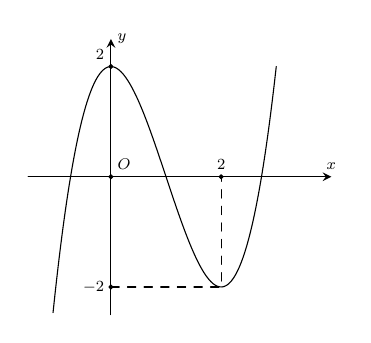
\begin{tikzpicture}[line join=round, line cap = round, >=stealth, scale=0.7,font=\footnotesize,transform shape]
            \draw[->] (-1.5,0) -- (4,0)node[above]{$x$};
            \draw[->] (0,-2.5) -- (0,2.5)node[right]{$y$};
            %\draw[-] (-1,-1.33) -- (3,-1.33) node[right]{$y=-\frac{4}{3}$};
            \draw[fill=black]
            (0,0) circle(1pt) node[above right]{$O$}
            (0,-2) circle(1pt) node[left]{$-2$}
            (2,0) circle(1pt) node[above]{$2$}
            (0,2) circle(1pt) node[above left]{$2$}
            ;
            \draw[dashed] (0,-2)--(2,-2)--(2,0);
            \draw[smooth,samples=100,domain=-1.05:3] plot(\x,{(\x)^3-3*(\x)^2+2});
        \end{tikzpicture}
    \end{center}
    \choice
    {\True $3$}
    {$0$}
    {$1$}
    {$2$}
    \loigiai{
        Ta có $3f(x)+4=0 \Leftrightarrow f(x)=-\dfrac{4}{3}.\quad (*)$\\
        \begin{center}
            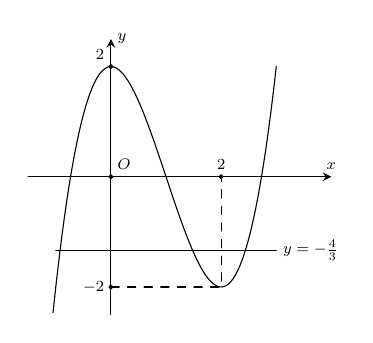
\begin{tikzpicture}[line join=round, line cap = round, >=stealth, scale=0.7,font=\footnotesize,transform shape]
                \draw[->] (-1.5,0) -- (4,0)node[above]{$x$};
                \draw[->] (0,-2.5) -- (0,2.5)node[right]{$y$};
                \draw[-] (-1,-1.33) -- (3,-1.33) node[right]{$y=-\frac{4}{3}$};
                \draw[fill=black]
                (0,0) circle(1pt) node[above right]{$O$}
                (0,-2) circle(1pt) node[left]{$-2$}
                (2,0) circle(1pt) node[above]{$2$}
                (0,2) circle(1pt) node[above left]{$2$}
                ;
                \draw[dashed] (0,-2)--(2,-2)--(2,0);
                \draw[smooth,samples=100,domain=-1.05:3] plot(\x,{(\x)^3-3*(\x)^2+2});
            \end{tikzpicture}
        \end{center}
        Số nghiệm của phương trình $(*)$ là số giao điểm của đồ thị hàm số $f(x)$ và đường thẳng nằm ngang $y=-\dfrac{4}{3}$. Quan sát hình vẽ, nhận thấy số giao điểm là $3$. Suy ra số nghiệm của phương trình là $3$.
    }
\end{ex}
\begin{ex}%[2D1B5-3]
    Cho hàm số $y=f(x)$ có đồ thị như hình. Tìm số nghiệm của phương trình $4f(x)-3=0$.
    \begin{center}
        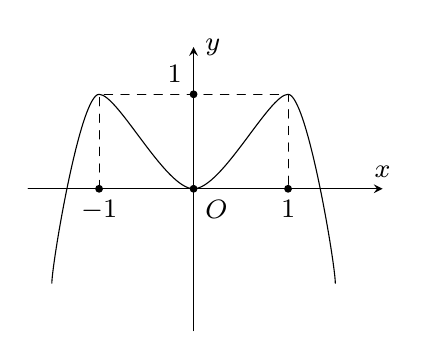
\begin{tikzpicture}[line join=round, line cap = round, >=stealth, scale=1.2,font=\footnotesize,transform shape]
            \draw[->] (-1.75,0) -- (2,0)node[above]{$x$};
            \draw[->] (0,-1.5) -- (0,1.5)node[right]{$y$};
            %\draw[-] (-1.5,0.75) -- (1.5,0.75) node[right]{$y=\frac{3}{4}$};
            \draw[fill=black]
            (0,0) circle(1pt) node[below right]{$O$}
            (-1,0) circle(1pt) node[below]{$-1$}
            (1,0) circle(1pt) node[below]{$1$}
            (0,1) circle(1pt) node[above left]{$1$}
            ;
            \draw[dashed] (-1,0)--(-1,1)--(1,1)--(1,0);
            \draw
            (-1.5,-1) .. controls +(90:.2) and +(180:.2) .. (-1,1)
            .. controls +(0:.2) and +(180:.3) .. (0,0)
            .. controls +(0:.3) and +(180:.2) .. (1,1)
            .. controls +(0:.2) and +(90:.2) .. (1.5,-1)
            ;
        \end{tikzpicture}
    \end{center}
    \choice
    {\True $4$}
    {$3$}
    {$2$}
    {$0$}
    \loigiai{
        Ta có $4f(x)-3=0 \Leftrightarrow f(x)=\dfrac{3}{4}.\quad (*)$
        \begin{center}
            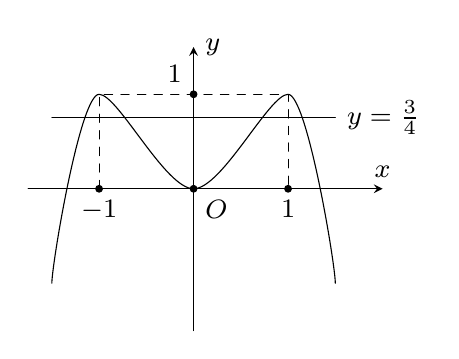
\begin{tikzpicture}[line join=round, line cap = round, >=stealth, scale=1.2,font=\footnotesize,transform shape]
                \draw[->] (-1.75,0) -- (2,0)node[above]{$x$};
                \draw[->] (0,-1.5) -- (0,1.5)node[right]{$y$};
                \draw[-] (-1.5,0.75) -- (1.5,0.75) node[right]{$y=\frac{3}{4}$};
                \draw[fill=black]
                (0,0) circle(1pt) node[below right]{$O$}
                (-1,0) circle(1pt) node[below]{$-1$}
                (1,0) circle(1pt) node[below]{$1$}
                (0,1) circle(1pt) node[above left]{$1$}
                ;
                \draw[dashed] (-1,0)--(-1,1)--(1,1)--(1,0);
                \draw
                (-1.5,-1) .. controls +(90:.2) and +(180:.2) .. (-1,1)
                .. controls +(0:.2) and +(180:.3) .. (0,0)
                .. controls +(0:.3) and +(180:.2) .. (1,1)
                .. controls +(0:.2) and +(90:.2) .. (1.5,-1)
                ;
            \end{tikzpicture}
        \end{center}
        Số nghiệm của phương trình $(*)$ là số giao điểm của đồ thị hàm số $f(x)$ và đường thẳng nằm ngang $y=\dfrac{3}{4}$. \\
        Quan sát hình vẽ, nhận thấy số giao điểm là $4$. Suy ra số nghiệm của phương trình là $4$.
    }
\end{ex}
\begin{ex}%[2D1B5-3]
    Cho hàm số $y=f(x)$ có đồ thị như hình. Tìm số nghiệm của phương trình $3f(x)-4=0$.
    \begin{center}
        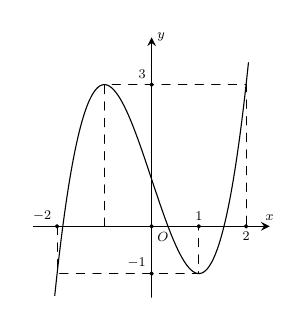
\begin{tikzpicture}[line join=round, line cap = round, >=stealth, scale=0.6,font=\footnotesize,transform shape]
            \draw[->] (-2.5,0) -- (2.5,0)node[above]{$x$};
            \draw[->] (0,-1.5) -- (0,4)node[right]{$y$};
            %\draw[-] (-2,1.33) -- (2.2,1.33) node[right]{$y=\frac{4}{3}$};
            \draw[fill=black]
            (0,0) circle(1pt) node[below right]{$O$}
            (0,3) circle(1pt) node[above left]{$3$}
            (2,0) circle(1pt) node[below]{$2$}
            (1,0) circle(1pt) node[above]{$1$}
            (-2,0) circle(1pt) node[above left]{$-2$}
            (0,-1) circle(1pt) node[above left]{$-1$}
            ;
            \draw[dashed]
            (-2,0)--(-2,-1)--(1,-1)--(1,0)
            (-1,0)--(-1,3)--(2,3)--(2,0)
            ;
            \draw[smooth,samples=100,domain=-2.05:2.05] plot(\x,{(\x)^3-3*(\x)+1});
        \end{tikzpicture}
    \end{center}
    \choice
    {$2$}
    {\True $3$}
    {$4$}
    {$1$}
    \loigiai{
        Ta có $3f(x)-4=0 \Leftrightarrow f(x)=\dfrac{4}{3}.\quad (*)$
        \begin{center}
            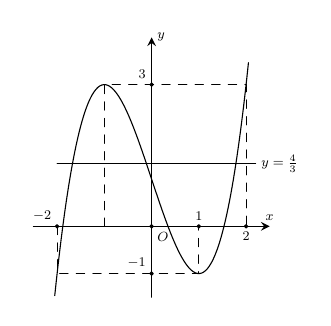
\begin{tikzpicture}[line join=round, line cap = round, >=stealth, scale=0.6,font=\footnotesize,transform shape]
                \draw[->] (-2.5,0) -- (2.5,0)node[above]{$x$};
                \draw[->] (0,-1.5) -- (0,4)node[right]{$y$};
                \draw[-] (-2,1.33) -- (2.2,1.33) node[right]{$y=\frac{4}{3}$};
                \draw[fill=black]
                (0,0) circle(1pt) node[below right]{$O$}
                (0,3) circle(1pt) node[above left]{$3$}
                (2,0) circle(1pt) node[below]{$2$}
                (1,0) circle(1pt) node[above]{$1$}
                (-2,0) circle(1pt) node[above left]{$-2$}
                (0,-1) circle(1pt) node[above left]{$-1$}
                ;
                \draw[dashed]
                (-2,0)--(-2,-1)--(1,-1)--(1,0)
                (-1,0)--(-1,3)--(2,3)--(2,0)
                ;
                \draw[smooth,samples=100,domain=-2.05:2.05] plot(\x,{(\x)^3-3*(\x)+1});
            \end{tikzpicture}
        \end{center}
        Số nghiệm của phương trình $(*)$ là số giao điểm của đồ thị hàm số $f(x)$ và đường thẳng nằm ngang $y=\dfrac{4}{3}$. Quan sát hình vẽ, nhận thấy số giao điểm là $3$. Suy ra số nghiệm của phương trình là $3$.
    }
\end{ex}
\begin{ex}%[2D1B5-3]
    Cho hàm số $y=f(x)$ có bảng biến thiên dưới. Tìm số nghiệm của phương trình $f(x)+3=0$.
    \begin{center}
        
\begin{tikzpicture}
            \tkzTabInit[nocadre=false,lgt=1.2,espcl=2,deltacl=0.6]
            {$x$ /0.6, $y'$ /0.6, $y$ /2}
            {$-\infty$,$-1$,$1$,$+\infty$}
            \tkzTabLine{,+,$0$,-,$0$,+,}
            \tkzTabVar{-/$-\infty$,+/$2$,-/$-3$,+/$+\infty$}
        \end{tikzpicture}
    \end{center}
    \choice
    {$0$}
    {$3$}
    {$1$}
    {\True $2$}
    \loigiai{
        Ta có $f(x)+3=0 \Leftrightarrow f(x)=-3.\quad (*)$\\
        Nhìn vào bảng biến thiên ta thấy đường thẳng $y=-3$ cắt đồ thị của hàm số $y=f(x)$ tại $2$ điểm.\\
        Vậy phương trình $(*)$ có $2$ nghiệm.
    }
\end{ex}
\begin{ex}%[2D1Y5-3]
    Cho hàm số $y=f(x)$ có bảng biến thiên dưới. Tìm số nghiệm của phương trình $f(x)=0$.
    \begin{center}
        
\begin{tikzpicture}
            \tkzTabInit[nocadre=false,lgt=1.2,espcl=2,deltacl=0.6]
            {$x$ /0.6, $y'$ /0.6, $y$ /2}
            {$-\infty$,$1$,$3$,$+\infty$}
            \tkzTabLine{,+,$0$,-,$0$,+,}
            \tkzTabVar{-/$-\infty$,+/$2$,-/$-1$,+/$+\infty$}
        \end{tikzpicture}
    \end{center}
    \choice
    {\True $3$}
    {$0$}
    {$1$}
    {$2$}
    \loigiai{
        Nhìn vào bảng biến thiên ta thấy đường thẳng $y=0$ cắt đồ thị của hàm số $y=f(x)$ tại $3$ điểm.\\
        Vậy phương trình $f(x)=0$ có $3$ nghiệm.
    }
\end{ex}
\begin{ex}%[2D1B5-3]
    Cho hàm số $y=f(x)$ có bảng biến thiên dưới. Tìm số nghiệm của phương trình $f(x)+1=0$.
    \begin{center}
        
\begin{tikzpicture}
            \tkzTabInit[nocadre=false,lgt=1.2,espcl=2,deltacl=0.6]
            {$x$ /0.6, $y'$ /0.6, $y$ /2}
            {$-\infty$,$1$,$3$,$+\infty$}
            \tkzTabLine{,+,$0$,-,d,+,}
            \tkzTabVar{-/$-\infty$,+/$2$,-/$-1$,+/$+\infty$}
        \end{tikzpicture}
    \end{center}
    \choice
    {$3$}
    {$0$}
    {$1$}
    {\True $2$}
    \loigiai{
        Ta có $f(x)+1=0\Leftrightarrow f(x)=-1.\quad (*)$\\
        Nhìn vào bảng biến thiên ta thấy đường thẳng $y=-1$ cắt đồ thị của hàm số $y=f(x)$ tại $2$ điểm.
        \begin{note}
            Ở đây nghiệm $x=3$ không thuộc tập xác định của $f'(x)$ nhưng vẫn thuộc tập xác định của $f(x)$ nên nghiệm $x=3$ vẫn được tính.
        \end{note}
        Vậy phương trình $(*)$ có $2$ nghiệm.
    }
\end{ex}
\begin{ex}%[2D1K5-3]
    Cho hàm số $y=f(x)$ có bảng biến thiên dưới. Tìm số nghiệm của phương trình $f^2(x)-4=0$.
    \begin{center}
        
\begin{tikzpicture}
            \tkzTabInit[nocadre=false,lgt=1.2,espcl=2,deltacl=0.6]
            {$x$ /0.6, $y'$ /0.6, $y$ /2}
            {$-\infty$,$-1$,$3$,$+\infty$}
            \tkzTabLine{,+,$0$,-,$0$,+,}
            \tkzTabVar{-/$-\infty$,+/$4$,-/$-2$,+/$+\infty$}
        \end{tikzpicture}
    \end{center}
    \choice
    {$3$}
    {\True $5$}
    {$1$}
    {$2$}
    \loigiai{
        Ta có $f^2(x)-4=0\Leftrightarrow\hoac{&f(x)=2 &(1)\\ &f(x)=-2. &(2)}$\\
        Nhìn vào bảng biến thiên ta thấy đường thẳng $y=2$ cắt đồ thị của hàm số $y=f(x)$ tại $3$ điểm. Suy ra phương trình $(1)$ có $3$ nghiệm.\\
        Nhìn vào bảng biến thiên ta thấy đường thẳng $y=-2$ cắt đồ thị của hàm số $y=f(x)$ tại $2$ điểm. Suy ra phương trình $(2)$ có $2$ nghiệm.\\
        Vậy phương trình $f^2(x)-4=0$ có $5$ nghiệm.
    }
\end{ex}
\begin{ex}%[2D1K5-3]
    Cho hàm số $y=f(x)$ có bảng biến thiên dưới. Tìm số nghiệm của phương trình $2f^2(x)-3f(x)+1=0$.
    \begin{center}
        
\begin{tikzpicture}
            \tkzTabInit[nocadre=false,lgt=1.2,espcl=2,deltacl=0.6]
            {$x$ /0.6, $y'$ /0.6, $y$ /2}
            {$-\infty$,$-1$,$1$,$+\infty$}
            \tkzTabLine{,+,$0$,-,$0$,+,}
            \tkzTabVar{-/$1$,+/$3$,-/$\frac{1}{3}$,+/$1$}
        \end{tikzpicture}
    \end{center}
    \choice
    {$6$}
    {$0$}
    {\True $3$}
    {$2$}
    \loigiai{
        Ta có $2f^2(x)-3f(x)+1=0\Leftrightarrow\hoac{&f(x)=1 &(1)\\ &f(x)=\dfrac{1}{2}. &(2)}$\\
        Nhìn vào bảng biến thiên với chú ý $\lim\limits_{x\to +\infty}f(x)=\lim\limits_{x\to -\infty}f(x)=1$, ta thấy đường thẳng $y=1$ cắt đồ thị của hàm số $y=f(x)$ tại duy nhất $1$ điểm nằm trong khoảng $(-1;1)$. Suy ra phương trình $(1)$ có $1$ nghiệm.\\
        Nhìn vào bảng biến thiên ta thấy đường thẳng $y=\dfrac{1}{2}$ cắt đồ thị của hàm số $y=f(x)$ tại $2$ điểm. Suy ra phương trình $(2)$ có $2$ nghiệm.\\
        Vậy phương trình $2f^2(x)-3f(x)+1=0$ có $3$ nghiệm.
    }
\end{ex}
\begin{ex}%[2D1B5-3]
    Cho đồ thị hàm số $y=x^3-3x+1$ như hình bên dưới. Tìm tất cả các giá trị của tham số $m$ để phương trình $x^3-3x-m=0$ có đúng $3$ nghiệm phân biệt.
    \begin{center}
        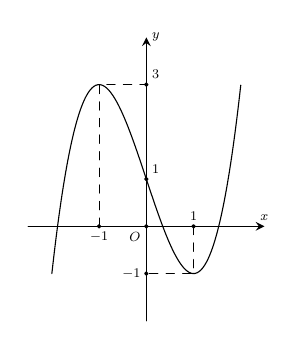
\begin{tikzpicture}[line join=round, line cap = round, >=stealth, scale=.6,font=\footnotesize,transform shape]
            \draw[->] (-2.5,0) -- (2.5,0)node[above]{$x$};
            \draw[->] (0,-2) -- (0,4)node[right]{$y$};
            %\draw[-] (-2,2) -- (2,2) node[right]{$y=m$};
            \draw[fill=black]
            (0,0) circle(1pt) node[below left]{$O$}
            (0,1) circle(1pt) node[above right]{$1$}
            (0,3) circle(1pt) node[above right]{$3$}
            (0,-1) circle(1pt) node[left]{$-1$}
            (-1,0) circle(1pt) node[below]{$-1$}
            (1,0) circle(1pt) node[above]{$1$}
            ;
            \draw[dashed]
            (-1,0)--(-1,3)--(0,3)
            (1,0)--(1,-1)--(0,-1)
            ;
            \draw[smooth,samples=100,domain=-2:2] plot(\x,{(\x)^3-3*(\x)+1});
        \end{tikzpicture}
    \end{center}
    \choice
    {$-2<m<3$}
    {\True $-2<m<2$}
    {$-2\le m<2$}
    {$-1<m<3$}
    \loigiai{
        Ta có $x^3-3x-m=0\Leftrightarrow x^3-3x+1=m+1$. \quad$(*)$\\
        Phương trình $(*)$ có đúng $3$ nghiệm phân biệt khi và chỉ khi đường thẳng $y=m+1$ cắt đồ thị hàm số $y=x^3-3x+1$ tại đúng $3$ điểm phân biệt.
        \begin{center}
            \begin{tikzpicture}[line join=round, line cap = round, >=stealth, scale=1,font=\footnotesize,transform shape]
                \draw[->] (-2.5,0) -- (2.5,0)node[above]{$x$};
                \draw[->] (0,-2) -- (0,4)node[right]{$y$};
                \draw[-] (-2,2) -- (2,2) node[right]{$y=m+1$};
                \draw[fill=black]
                (0,0) circle(1pt) node[below left]{$O$}
                (0,1) circle(1pt) node[above right]{$1$}
                (0,3) circle(1pt) node[above right]{$3$}
                (0,-1) circle(1pt) node[left]{$-1$}
                (-1,0) circle(1pt) node[below]{$-1$}
                (1,0) circle(1pt) node[above]{$1$}
                ;
                \draw[dashed]
                (-1,0)--(-1,3)--(0,3)
                (1,0)--(1,-1)--(0,-1)
                ;
                \draw[smooth,samples=100,domain=-2:2] plot(\x,{(\x)^3-3*(\x)+1});
            \end{tikzpicture}
        \end{center}
        Nhìn vào đồ thị ta thấy điều này xảy ra khi và chỉ khi $-1<m+1<3 \Leftrightarrow -2<m<2$.\\
        Vậy phương trình đã cho có đúng $3$ nghiệm phân biệt khi và chỉ khi $-2<m<2$.
    }
\end{ex}
\begin{ex}%[2D1B5-3]
    Cho đồ thị hàm số $y=-x^3+3x^2-4$ như hình bên dưới. Tìm tất cả các giá trị của tham số $m$ để phương trình $x^3-3x^2+m+5=0$ có đúng $2$ nghiệm phân biệt.
    \begin{center}
        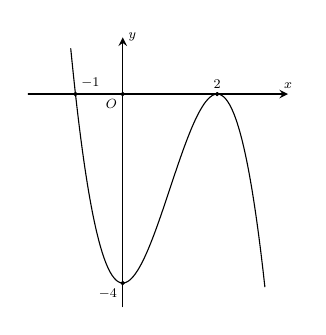
\begin{tikzpicture}[line join=round, line cap = round, >=stealth, scale=.6,font=\footnotesize,transform shape]
            \draw[->] (-2,0) -- (3.5,0)node[above]{$x$};
            \draw[->] (0,-4.5) -- (0,1.2)node[right]{$y$};
            %\draw[-] (-1,-4) -- (3.2,-4) node[right]{$y=m$};
            \draw[fill=black]
            (0,0) circle(1pt) node[below left]{$O$}
            (0,-4) circle(1pt) node[below left]{$-4$}
            (-1,0) circle(1pt) node[above right]{$-1$}
            (2,0) circle(1pt) node[above]{$2$}
            ;
            \draw[smooth,samples=100,domain=-1.1:3.01] plot(\x,{-(\x)^3+3*(\x)^2-4});
        \end{tikzpicture}
    \end{center}
    \choice
    {\True $m=-1$ hoặc $m=-5$}
    {$m=4$}
    {$0<m<4$}
    {$m=4$}
    \loigiai{
        Ta có $x^3-3x^2+m+5=0\Leftrightarrow -x^3+3x^2-4=m+1$. \quad$(*)$
        Phương trình $(*)$ có đúng $2$ nghiệm phân biệt khi và chỉ khi đường thẳng $y=m+1$ cắt đồ thị hàm số $y=-x^3+3x^2-4$ tại đúng $2$ điểm phân biệt.
        \begin{center}
            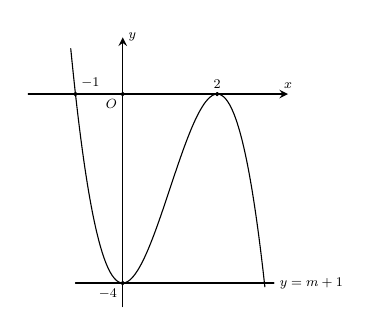
\begin{tikzpicture}[line join=round, line cap = round, >=stealth, scale=.6,font=\footnotesize,transform shape]
                \draw[->] (-2,0) -- (3.5,0)node[above]{$x$};
                \draw[->] (0,-4.5) -- (0,1.2)node[right]{$y$};
                \draw[-] (-1,-4) -- (3.2,-4) node[right]{$y=m+1$};
                \draw[fill=black]
                (0,0) circle(1pt) node[below left]{$O$}
                (0,-4) circle(1pt) node[below left]{$-4$}
                (-1,0) circle(1pt) node[above right]{$-1$}
                (2,0) circle(1pt) node[above]{$2$}
                ;
                \draw[smooth,samples=100,domain=-1.1:3.01] plot(\x,{-(\x)^3+3*(\x)^2-4});
            \end{tikzpicture}
        \end{center}
        Nhìn vào đồ thị ta thấy điều này xảy ra khi và chỉ khi $\hoac{&m+1=0\\ &m+1=-4} \Leftrightarrow\hoac{&m=-1\\ &m=-5.}$\\
        Vậy phương trình đã cho có đúng $2$ nghiệm phân biệt khi và chỉ khi $m=-1$ hoặc $m=-5$.
    }
\end{ex}
\begin{ex}%[2D1B5-3]
    Cho đồ thị hàm số $y=f(x)$ như hình bên dưới. Tìm tất cả các giá trị của tham số $m$ để phương trình $f(x)+1=m$ có đúng $3$ nghiệm phân biệt.
    \begin{center}
        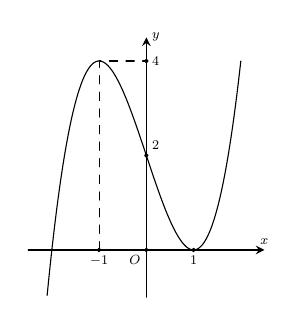
\begin{tikzpicture}[line join=round, line cap = round, >=stealth, scale=1.2,font=\footnotesize,transform shape, scale=.5]
            \draw[->] (-2.5,0) -- (2.5,0)node[above]{$x$};
            \draw[->] (0,-1) -- (0,4.5)node[right]{$y$};
            %\draw[-] (-2.5,1) -- (2,1) node[right]{$y=m-1$};
            \draw[fill=black]
            (0,0) circle(1pt) node[below left]{$O$}
            (0,2) circle(1pt) node[above right]{$2$}
            (0,4) circle(1pt) node[right]{$4$}
            (-1,0) circle(1pt) node[below]{$-1$}
            (1,0) circle(1pt) node[below]{$1$}
            ;
            \draw[dashed]
            (-1,0)--(-1,4)--(0,4)
            ;
            \draw[smooth,samples=100,domain=-2.1:2] plot(\x,{(\x)^3-3*(\x)+2});
        \end{tikzpicture}
    \end{center}
    \choice
    {$0<m<5$}
    {\True $1<m<5$}
    {$-1<m<4$}
    {$0<m<4$}
    \loigiai{
        Ta có $f(x)+1=m \Leftrightarrow f(x)=m-1$. \quad $(*)$\\
        Phương trình $(*)$ có đúng $3$ nghiệm phân biệt khi và chỉ khi đường thẳng $y=m-1$ cắt đồ thị hàm số $y=f(x)$ tại đúng $3$ điểm phân biệt.
        \begin{center}
            \begin{tikzpicture}[line join=round, line cap = round, >=stealth, scale=1.2,font=\footnotesize,transform shape]
                \draw[->] (-2.5,0) -- (2.5,0)node[above]{$x$};
                \draw[->] (0,-1) -- (0,4.5)node[right]{$y$};
                \draw[-] (-2.5,1) -- (2,1) node[right]{$y=m-1$};
                \draw[fill=black]
                (0,0) circle(1pt) node[below left]{$O$}
                (0,2) circle(1pt) node[above right]{$2$}
                (0,4) circle(1pt) node[right]{$4$}
                (-1,0) circle(1pt) node[below]{$-1$}
                (1,0) circle(1pt) node[below]{$1$}
                ;
                \draw[dashed]
                (-1,0)--(-1,4)--(0,4)
                ;
                \draw[smooth,samples=100,domain=-2.1:2] plot(\x,{(\x)^3-3*(\x)+2});
            \end{tikzpicture}
        \end{center}
        Nhìn vào đồ thị ta thấy điều này xảy ra khi và chỉ khi $0<m-1<4 \Leftrightarrow 1<m<5$.\\
        Vậy phương trình đã cho có đúng $3$ nghiệm phân biệt khi và chỉ khi $1<m<5$.
    }
\end{ex}
\begin{ex}%[2D1B5-3]
    Cho đồ thị hàm số $y=f(x)$ như hình bên dưới. Tìm tất cả các giá trị của tham số $m$ để phương trình $f(x)=m$ có đúng $3$ nghiệm phân biệt thuộc đoạn $[-2;1]$.
    \begin{center}
        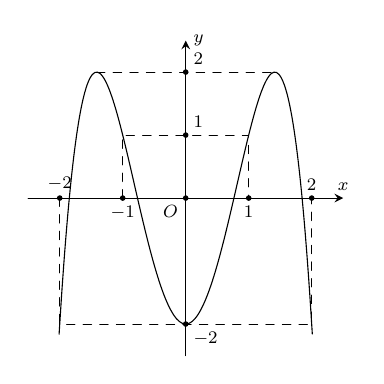
\begin{tikzpicture}[line join=round, line cap = round, >=stealth, scale=.8,font=\footnotesize,transform shape]
            \pgfmathsetmacro\a{sqrt(2)}
            \draw[->] (-2.5,0) -- (2.5,0)node[above]{$x$};
            \draw[->] (0,-2.5) -- (0,2.5)node[right]{$y$};
            %\draw[-] (-2.2,-1) -- (.75,-1) node[right]{$y=m$};
            \draw[fill=black]
            (0,0) circle(1pt) node[below left]{$O$}
            (0,2) circle(1pt) node[above right]{$2$}
            (0,1) circle(1pt) node[above right]{$1$}
            (0,-2) circle(1pt) node[below right]{$-2$}
            (2,0) circle(1pt) node[above]{$2$}
            (-2,0) circle(1pt) node[above]{$-2$}
            (-1,0) circle(1pt) node[below]{$-1$}
            (1,0) circle(1pt) node[below]{$1$}
            ;
            \draw[dashed]
            (-\a,2)--(\a,2)
            (-2,0)--(-2,-2)--(2,-2)--(2,0)
            (-1,0)--(-1,1)--(1,1)--(1,0)
            ;
            \draw[smooth,samples=100,domain=-2.01:2.01] plot(\x,{-(\x)^4+4*(\x)^2-2});
        \end{tikzpicture}
    \end{center}
    \choice
    {$-2<m<0$}
    {$-2\le m<1$}
    {\True $-2<m\le 1$}
    {$-2<m\le 0$}
    \loigiai{
        Phương trình $f(x)=m$ có đúng $3$ nghiệm phân biệt thuộc đoạn $[-2;1]$ khi và chỉ khi đường thẳng $y=m$ cắt phần đồ thị ứng với $x\in [-2;1]$ của đồ thị hàm số $y=f(x)$ tại đúng $3$ điểm phân biệt.
        \begin{center}
            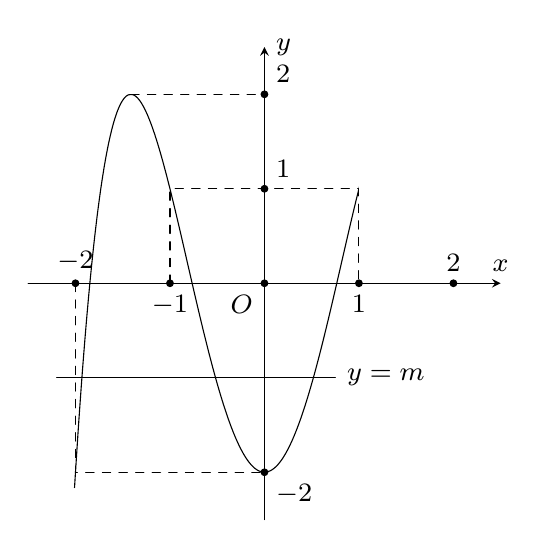
\begin{tikzpicture}[line join=round, line cap = round, >=stealth, scale=1.2,font=\footnotesize,transform shape]
                \pgfmathsetmacro\a{sqrt(2)}
                \draw[->] (-2.5,0) -- (2.5,0)node[above]{$x$};
                \draw[->] (0,-2.5) -- (0,2.5)node[right]{$y$};
                \draw[-] (-2.2,-1) -- (.75,-1) node[right]{$y=m$};
                \draw[fill=black]
                (0,0) circle(1pt) node[below left]{$O$}
                (0,2) circle(1pt) node[above right]{$2$}
                (0,1) circle(1pt) node[above right]{$1$}
                (0,-2) circle(1pt) node[below right]{$-2$}
                (2,0) circle(1pt) node[above]{$2$}
                (-2,0) circle(1pt) node[above]{$-2$}
                (-1,0) circle(1pt) node[below]{$-1$}
                (1,0) circle(1pt) node[below]{$1$}
                ;
                \draw[dashed]
                (-\a,2)--(0,2)
                (-2,0)--(-2,-2)--(0,-2)
                (-1,0)--(-1,1)--(1,1)--(1,0)
                ;
                \clip (-2.5,-2.5) rectangle (1,2);
                \draw[smooth,samples=100,domain=-2.01:2.01] plot(\x,{-(\x)^4+4*(\x)^2-2});
            \end{tikzpicture}
        \end{center}
        Nhìn vào đồ thị ta thấy điều này xảy ra khi và chỉ khi $-2<m\le 1$.\\
        Vậy phương trình đã cho có đúng $3$ nghiệm phân biệt thuộc đoạn $[-2;1]$ khi và chỉ khi $-2<m\le 1$.
    }
\end{ex}
\begin{ex}%[2D1B5-3]
    \immini
    {
        Cho hàm số $y=f(x)$ có đồ thị như hình vẽ. Số nghiệm của phương trình $2f(x)-3=0$ là
        \haicot
        {$2$}
        {$1$}
        {$0$}
        {\True $3$}
    }
    {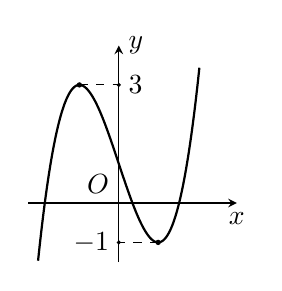
\begin{tikzpicture}[smooth,samples=300,scale=0.5,>=stealth]
            \draw[->] (-2.3,0)--(3,0) node[below]{$x$};
            \draw[->] (0,-1.5)--(0,4) node[right]{$y$};
            \draw (0,0) node[above left]{$O$};
            \draw[thick,domain=-2.05:2.05] plot(\x,{1*((\x)^3)-3*(\x)+1});
            \draw[fill=black] (0,3) circle(1pt) (-1,3) circle(1.5pt) (0,-1) circle(1pt) (1,-1) circle(1.5pt);
            \draw[dashed] (1,-1)--(0,-1)node[left]{$-1$} (-1,3)--(0,3)node[right]{$3$};
        \end{tikzpicture}
    }
    \loigiai{
        Ta có $2f(x)-3=0\Leftrightarrow f(x)=\dfrac{3}{2}$.\\
        Từ đồ thị suy ra phương trình có $3$ nghiệm phân biệt.
    }
\end{ex}
\begin{ex}%[2D1B5-3]
    \immini
    {Cho hàm số $f(x)=ax^3 +bx^2 +cx +d$ $(d\ne 0)$ có đồ thị như hình vẽ bên. Số nghiệm của phương trình $3f(x) -1 =0$ bằng
        \haicot
        {$0$}
        {\True $1$}
        {$2$}
        {$3$}
    }
    {\hspace{1cm}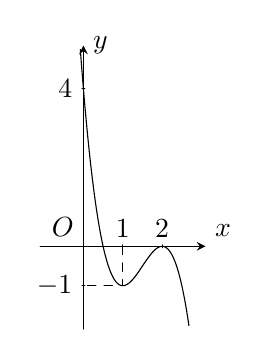
\begin{tikzpicture}[line join=round, line cap=round,>=stealth,scale=0.5]
            \tikzset{label style/.style={font=\footnotesize}}
            \draw[->] (-1.1,0)--(3.1,0) node[above right] {$x$};
            \draw[->] (0,-2.1)--(0,5.1) node[right] {$y$};
            \draw (0,0) node [above left] {$O$};
            \foreach \x in {1,2}
            \draw[thin] (\x,1pt)--(\x,-1pt) node [above] {$\x$};
            \foreach \y in {-1,4}
            \draw[thin] (1pt,\y)--(-1pt,\y) node [left] {$\y$};
            %\draw[dashed,thin](-1,0)--(-1,3)--(0,3);
            \draw[dashed,thin](1,0)--(1,-1)--(0,-1);
            \begin{scope}
                \clip (-1,-2) rectangle (3,5);
                \draw[samples=200,domain=-1:3,smooth,variable=\x] plot (\x,{-2*((\x)^3)+9*((\x)^2)+-12*(\x)+4});
            \end{scope}
    \end{tikzpicture}}
    \loigiai{
        Ta có $3f(x)-1=0 \Leftrightarrow f(x) = \dfrac{1}{3}$.\\
        Khi đó số giao điểm của đồ thị $y=f(x)$ và đường thẳng $y=\dfrac{1}{3}$ chính là số nghiệm của phương trình $3f(x) -1=0$. Dựa vào đồ thị ta có số nghiệm của phương trình là 1.}
\end{ex}
\begin{ex}%[2D1B5-3]
    \immini{Cho hàm số $y = f(x)$ có bảng biến thiên như sau. Số giao điểm của đồ thị hàm số $y = f(x)$ với trục hoành là
        \choice
        {$ 1$}
        {$ 0$}
        {$ 2 $}
        {\True $ 3 $}}{
        
\begin{tikzpicture}
            \tkzTabInit[lgt=1,espcl=1.8]
            {$x$/0.6, $y’$/0.6, $y$/1.6}
            {$-\infty$,$0$,$1$,$+\infty$}
            \tkzTabLine{ ,-,$0$,+,$0$,-, }
            \tkzTabVar{+/$+\infty$,-/$-1$,+/$3$,-/$-\infty$}
    \end{tikzpicture}}
    \loigiai{
        Dựa vào bảng biến thiên thì đồ thị hàm số $y = f(x)$ và trục hoành có $3$ điểm chung.
    }
\end{ex}
\begin{ex}%[2D1B5-3]
    \immini{Cho hàm số $y=f(x)$ liên tục trên $(-\infty;+\infty)$ và có bảng biến thiên như hình bên. Số nghiệm thực của phương trình $2\big|f(x)\big|=7$ bằng
        \choice
        {$3$}
        {\True $2$}
        {$4$}
        {$2$}
    }{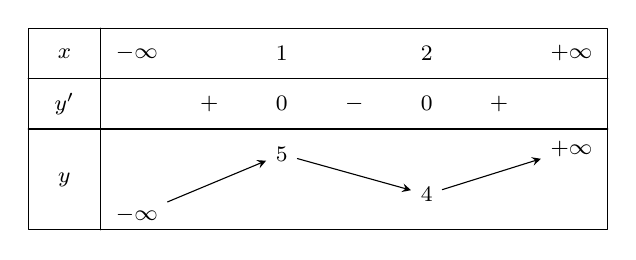
\begin{tikzpicture}[>=stealth,line join=round,line cap=round,font=\footnotesize,scale=.8]
            \begin{scope}[xscale=1.15,yscale=0.8]
                \begin{scope}[shift={(-0.5,0.5)}]
                    \def\a{8}
                    \def\b{4}
                    \draw (0,0)rectangle +(\a,-\b)
                    (1,0)--+(-90:\b)
                    (0,-1)--+(0:\a)
                    (0,-2)--+(0:\a)
                    ;
                \end{scope}
                \draw
                (0,0)node{$x$}++(0:1)node{$-\infty$}++(0:2)node{$1$}++(0:2)node{$2$}
                ++(0:2)node{$+\infty$}
                (0,-1)node{$y'$}	++(0:2)node{$+$}++(0:1)node{$0$}++(0:1)node{$-$}++(0:1)node{$0$}++(0:1)node{$+$}
                (0,-2.5)node{$y$}
                (1,-3.2) node (A) {$-\infty$}
                (3,-2)node (B) {$5$}
                (5,-2.8) node (C){$4$}
                (7,-1.9)node (D){$+\infty$}
                ;
                \draw[->] (A)--(B);
                \draw[->] (B)--(C);
                \draw[->] (C)--(D);
            \end{scope}
    \end{tikzpicture}}
    \loigiai{
    }
\end{ex}
\begin{ex}%[2D1K5-3]
    \immini{Cho hàm số $y=f(x)$ liên tục trên $\mathbb{R}\setminus\{0\}$ và có bảng biến thiên như hình bên. Hỏi phương trình $3|f(x)|-10=0$ có bao nhiêu nghiệm?
        \choice
        {$2$ nghiệm}
        {$4$ nghiệm}
        {\True $3$ nghiệm}
        {$1$ nghiệm}
    }{
        
\begin{tikzpicture}
            \tikzset{double style/.append style = {draw=\tkzTabDefaultWritingColor,double=\tkzTabDefaultBackgroundColor,double distance=2pt}}
            \tkzTabInit[nocadre=false,lgt=1.2,espcl=1.7,deltacl=0.6]
            {$x$ /.6,$f'(x)$ /.6,$f(x)$ /1.7}{$-\infty$,$0$,$1$,$+\infty$}
            \tkzTabLine{,-,d,-,0,+,}
            \tkzTabVar{+/$2$,-D+/$-\infty$/+$\infty$,-/$3$,+/$+\infty$}
    \end{tikzpicture}}
    \loigiai
    {
        Từ bảng biến thiên đề bài, ta có bảng biến thiên của hàm số $y=|f(x)|$ như sau
        \begin{center}
            
\begin{tikzpicture}
                \tkzTabInit[nocadre=false,lgt=1.3,espcl=2.5,deltacl=0.6]
                {$x$ /.6,$f'(x)$ /.6,$|f(x)|$ /2}{$-\infty$,,$0$,$1$,$+\infty$}
                \tkzTabLine{,,-,,d,-,0,+,}
                \tkzTabVar{+/$2$,-/$0$,+D+/$+\infty$/+$\infty$,-/$3$,+/$+\infty$}
            \end{tikzpicture}
        \end{center}
        Ta có $3|f(x)|-10=0\Leftrightarrow |f(x)|=\dfrac{10}{3}.\qquad(1)$\\
        Số nghiệm của phương trình (1) bằng số giao điểm của đồ thị $y=|f(x)|$ và đường thẳng $y=3$.\\
        Dựa vào bảng biến thiên trên, suy ra phương trình (1) có $3$ nghiệm.
    }
\end{ex}
\begin{ex}%[2D1K5-3]
    \immini{Cho hàm số $y = f(x)$ xác định và liên tục trên $\mathbb{R}$, có bảng biến thiên như sau. Số nghiệm của phương trình $2[f(x)]^2- 3 f(x)+ 1 = 0$ là
        \choice
        {$2$}
        {\True $3$}
        {$6$}
        {$0$}}
    {
\begin{tikzpicture}[scale=0.8]
            \tkzTabInit[espcl=2.3,lgt=1.2,deltacl=0.6]
            {$x$/0.6,$y'$/0.6,$y$/2}
            {$-\infty$,$-1$,$1$,$+\infty$}
            \tkzTabLine{,+,0,-,0,+,}
            \tkzTabVar{-/$1$,+/$3$,-/$\dfrac{1}{3}$,+/$1$}
    \end{tikzpicture}}
    \loigiai{
        Ta có $ 2[f(x)]^2- 3 f(x)+ 1 = 0\Leftrightarrow \left[\begin{array}{l}{f(x)= 1}\\{f(x)= \dfrac{1}{2}.}\end{array}\right.$\\
        Phương trình $f(x)= 1$ có duy nhất nghiệm $ x_0 $.\\
        Phương trình $f(x)= \dfrac{1}{2}$ có $2$ nghiệm phân biệt khác $x_{0}$. Vậy phương trình có ba nghiệm.
    }
\end{ex}
\begin{ex}
    \immini{Cho hàm số $f(x)$ có bảng biến thiên như hình bên. Tìm tất cả các giá trị thực của tham số $m$ để phương trình $f(x)=m+1$ có ba nghiệm thực phân biệt.
        \choice
        {$-3\le m \le 3$}
        {$-2\le m \le 4$}
        {$-2<m<4$}
        {\True $-3<m<3$}
    }{
        
\begin{tikzpicture}
            \tkzTabInit[nocadre=false,lgt=1,espcl=1.9,deltacl=0.6]
            {$x$ /0.6, $y'$ /0.6, $y$ /1.6}
            {$-\infty$,$-1$,$3$,$+\infty$}
            \tkzTabLine{,+,$0$,-,$0$,+,}
            \tkzTabVar{-/$-\infty$,+/$4$,-/$-2$,+/$+\infty$}
    \end{tikzpicture}}
    \loigiai{
        Dựa vào bảng biến thiên phương trình $f(x)=m+1$ có ba nghiệm thực phân biệt khi
        \begin{center}
            $-2<m+1<4 \Leftrightarrow -3<m<3$.
        \end{center}
    }
\end{ex}
\begin{ex}
    \immini{Cho hàm số $y=f(x)$ có bảng biến thiên như hình bên. Phương trình $f(4x-x^2)-2=0$ có bao nhiêu nghiệm thực?
        \choice
        {$2$}
        {$6$}
        {$0$}
        {\True $4$}
    }{
        
\begin{tikzpicture}
            \tkzTabInit[nocadre=false,lgt=1.2,espcl=2.2,deltacl=0.6]
            {$x$ /0.6,$y’$ /0.6,$y$ /1.6}
            {$-\infty$ ,$0$ , $4$, $+\infty$}
            \tkzTabLine{,-,0,+,0,-}
            \tkzTabVar{+/ $+\infty $ / , -/ $-1$ /,+/ $3$/ , -/ $-\infty$ /}
    \end{tikzpicture} }
    \loigiai{
        Đặt $t=4x-x^2$. Khi đó $t=-(x-2)^2+4 \leq 4$.\\
        Từ mỗi giá trị $t<4$ ta tìm được hai giá trị $x$. Với $t=4$ ta tìm được $x=2$.\\
        Từ bảng biến thiên, ta thấy phương trình $f(t)=2 \Leftrightarrow \left [ \begin{aligned} &t=\alpha \in (-\infty;0)\\
            &t=\beta \in (0;4) \\
            &t=\gamma \in (4;+\infty) \end{aligned} \right.$\\
        Vậy phương trình $f(4x-x^2)-2=0$ có $4$ nghiệm.
    }
\end{ex}
\begin{ex}%[2D1K5-3]
    Cho đồ thị hàm số $y=f(x)$ như hình bên dưới. Hỏi phương trình $f(x)=x$ có bao nhiêu nghiệm?
    \begin{center}
        \begin{tikzpicture}[line join=round, line cap = round, >=stealth, scale=1.2,font=\footnotesize,transform shape]
            \pgfmathsetmacro\a{sqrt(2)}
            \draw[->] (-1.5,0) -- (3.25,0)node[above]{$x$};
            \draw[->] (0,-.5) -- (0,2.75)node[right]{$y$};
            %\draw[-] (-.5,-.5) -- (2.5,2.5) node[right]{$y=x$};
            \draw[fill=black]
            (0,0) circle(1pt) node[below right]{$O$}
            (2,0) circle(1pt) node[below]{$1$}
            (0,2) circle(1pt) node[above left]{$1$}
            ;
            \draw[dashed]
            (2,0)--(2,2)--(0,2)
            ;
            \draw[smooth,samples=100,domain=-1.1:3.1] plot(\x,{-(\x)^3/2+3*(\x)^2/2});
        \end{tikzpicture}
    \end{center}
    \choice
    {$0$}
    {$1$}
    {$2$}
    {\True $3$}
    \loigiai{
        Vẽ đồ thị của hàm số $y=f(x)$ và $y=x$ trên cùng một đồ thị như hình dưới đây.
        \begin{center}
            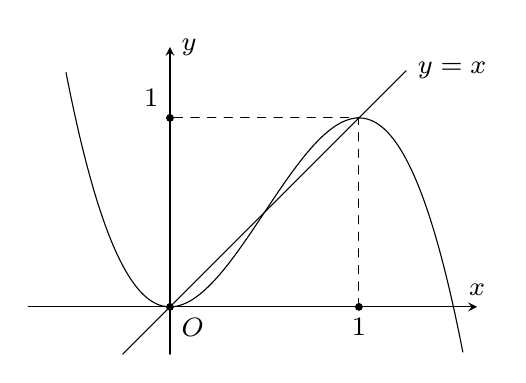
\begin{tikzpicture}[line join=round, line cap = round, >=stealth, scale=1.2,font=\footnotesize,transform shape]
                \pgfmathsetmacro\a{sqrt(2)}
                \draw[->] (-1.5,0) -- (3.25,0)node[above]{$x$};
                \draw[->] (0,-.5) -- (0,2.75)node[right]{$y$};
                \draw[-] (-.5,-.5) -- (2.5,2.5) node[right]{$y=x$};
                \draw[fill=black]
                (0,0) circle(1pt) node[below right]{$O$}
                (2,0) circle(1pt) node[below]{$1$}
                (0,2) circle(1pt) node[above left]{$1$}
                ;
                \draw[dashed]
                (2,0)--(2,2)--(0,2)
                ;
                \draw[smooth,samples=100,domain=-1.1:3.1] plot(\x,{-(\x)^3/2+3*(\x)^2/2});
            \end{tikzpicture}
        \end{center}
        Nhìn vào đồ thị ta thấy đường thẳng $y=x$ cắt đồ thị hàm số $y=f(x)$ tại $3$ điểm.\\
        Vậy phương trình đã cho có $3$ nghiệm.
    }
\end{ex}
\begin{ex}%[2D1B5-3]
    Cho bảng biến thiên của hàm số $y=f(x)$ như hình bên dưới. Tìm tất cả các giá trị của tham số $m$ để phương trình $f(x)=m$ có $3$ nghiệm phân biệt.
    \begin{center}
        
\begin{tikzpicture}
            \tkzTabInit[nocadre=false,lgt=1.2,espcl=2,deltacl=0.6]
            {$x$ /0.6, $y'$ /0.6, $y$ /2}
            {$-\infty$,$-1$,$3$,$+\infty$}
            \tkzTabLine{,+,$0$,-,$0$,+,}
            \tkzTabVar{-/$-\infty$,+/$4$,-/$-2$,+/$+\infty$}
        \end{tikzpicture}
    \end{center}
    \choice
    {$m<-2$}
    {\True $-2<m<4$}
    {$-2\le m\le 4$}
    {$m>4$}
    \loigiai{
        Phương trình $f(x)=m$ có đúng $3$ nghiệm phân biệt khi và chỉ khi đường thẳng $y=m$ cắt đồ thị hàm số $y=f(x)$ tại đúng $3$ điểm phân biệt.\\
        Nhìn vào bảng biến thiên ta thấy điều này xảy ra khi và chỉ khi $-2<m<4$.\\
        Vậy phương trình đã cho có đúng $3$ nghiệm phân biệt khi và chỉ khi $-2<m<4$.
    }
\end{ex}
\begin{ex}%[2D1B5-3]
    Cho bảng biến thiên của hàm số $y = f(x)$. Tìm tất cả các giá trị của tham số $m$ để phương trình $f(x) - 1 = 2m$ có ba nghiệm phân biệt?
    \begin{center}
        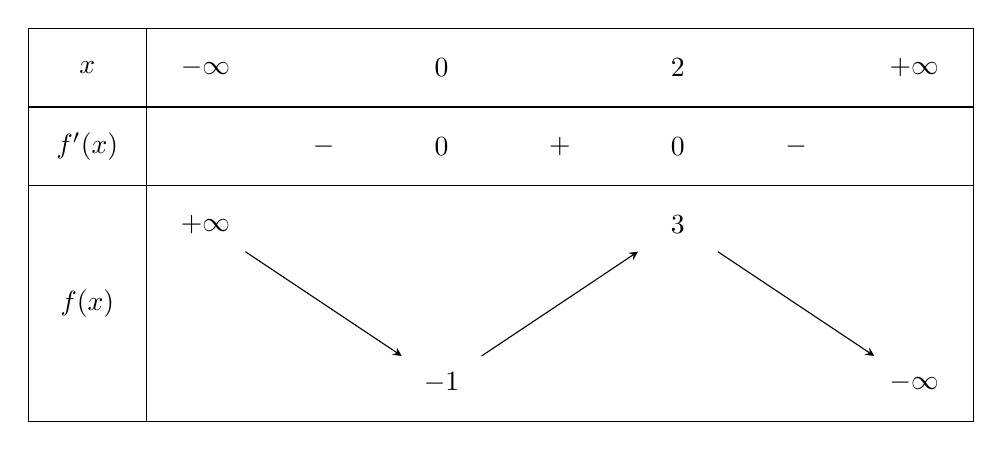
\begin{tikzpicture}[>=stealth,yscale=1,xscale=1.5]
            \def\c{7}%số cột
            \def\d{4}%số dòng
            \foreach \x in {0,...,\c}{
                \foreach \y in {0,...,-\d}
                \pgfmathsetmacro{\yy}{int(abs(\y))}
                \node[gray!0,minimum size=1cm] at (\x,\y) (\x\yy) {\x\yy};
            }
            \draw[shift={(-0.5,0.5)}]
            (0,0) rectangle (\c+1,-\d-1)
            (0,-1)--(\c+1,-1)
            (0,-2)--(\c+1,-2)
            (1,0)--(1,-\d-1);
            \path
            (00) node {$x$}
            (01) node {$f'(x)$}
            (03) node {$f(x)$}
            (10) node {$-\infty$}
            (30) node {$0$}
            (50) node {$2$}
            (70) node {$+\infty$}
            (21) node {$-$}
            (31) node {$0$}
            (41) node {$+$}
            (51) node {$0$}
            (61) node {$-$}
            (12) node {$+\infty$}
            (34) node {$-1$}
            (52) node {$3$}
            (74) node {$-\infty$}
            ;
            \draw[->] (12)--(34);
            \draw[->] (34)--(52);
            \draw[->] (52)--(74);
        \end{tikzpicture}
    \end{center}
    \choice
    {$-1 < m < 3$}
    {$-\dfrac{1}{2} < m < \dfrac{1}{2}$}
    {\True $0 < m < 2$}
    {$-1 < m < 1$}
    \loigiai{Theo giả thiết $f(x) - 1 = 2m \Leftrightarrow f(x) = 2m + 1$. Từ bảng biến thiên ta thấy rằng để phương trình có ba nghiệm phân biệt thì $2m - 1 \in (-1, 3)$. Từ đây suy ra $m \in (0, 2)$.
    }
\end{ex}

\begin{ex}%[2D1B5-3]
    Cho bảng biến thiên của hàm số $y = f(x)$. Tìm tất cả các giá trị của tham số $m$ để phương trình $f(x) = m$ có $3$ nghiệm phân biệt?
    \begin{center}
        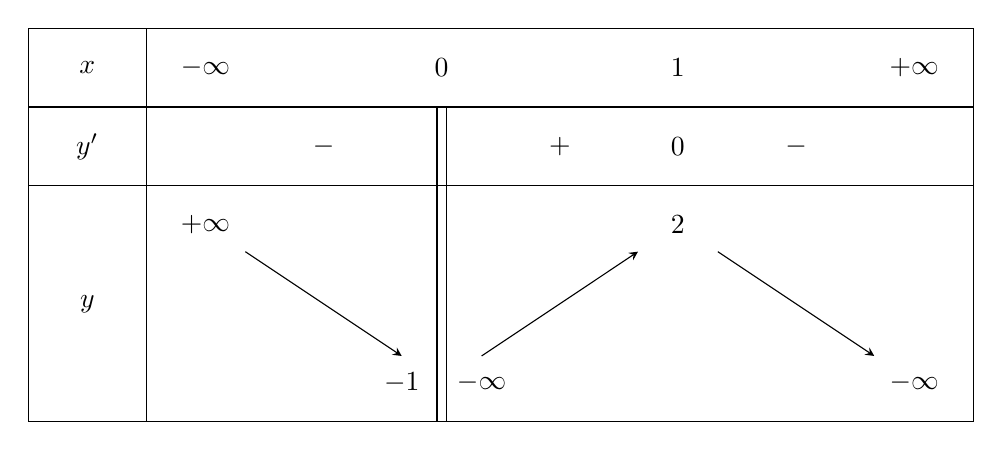
\begin{tikzpicture}[yscale=1,xscale=1.5]
            \def\c{7}%số cột
            \def\d{4}%số dòng
            \foreach \x in {0,...,\c}{
                \foreach \y in {0,...,\d}
                \path[yscale=-1] (\x,\y) node[gray!0,minimum size=1cm] (\x\y) {\x\y};
            }
            \path
            foreach \x/\t in {0/x,1/-\infty,3/0,5/1,7/+\infty} {(\x0) node {$\t$}}
            foreach \x/\t in {0/y',2/-,4/+,5/0,6/-} {(\x1) node {$\t$}}
            foreach \x/\t in {03/y,12/+\infty,34.west/-1,34.east/-\infty,52/2,74/-\infty} {(\x) node {$\t$}}
            ;
            \foreach \a/\b in {12/34,34/52,52/74} \draw[->,>=stealth] (\a)--(\b);
            \draw[double distance=3pt] (31.north)--(34.south);
            \draw[shift={(-0.5,0.5)}] (0,0) rectangle (\c+1,-\d-1)
            (0,-1)--(\c+1,-1) (0,-2)--(\c+1,-2) (1,0)--(1,-\d-1);
        \end{tikzpicture}
    \end{center}
    \choice
    {$m \in \left[ -1; 2\right]$}
    {\True $m \in \left( -1; 2\right)$}
    {$m \in \left[ -1; 2\right]$}
    {$m \in \left( -\infty; 2\right]$}
    \loigiai{Xét phương trình $f(x) = m$.
        Để phương trình có ba nghiệm phân biệt thì $-1 < m < 2$.
    }
\end{ex}
\begin{ex}%[2D1B5-3]
    Cho bảng biến thiên của hàm số $y = f(x)$. Tìm tất cả các giá trị của tham số $m$ để phương trình $f(x) = m$ có $3$ nghiệm phân biệt?
    \begin{center}
        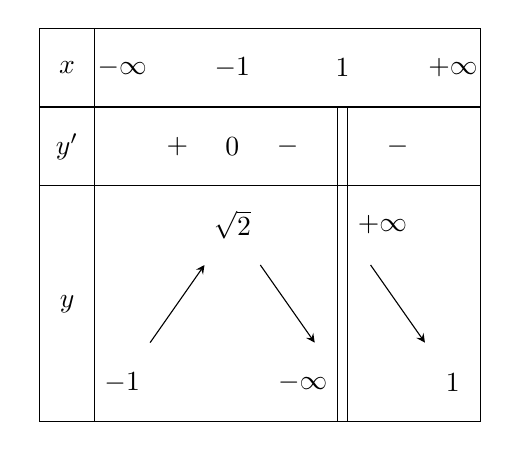
\begin{tikzpicture}[yscale=1,xscale=.7]
            \def\c{7}%số cột
            \def\d{4}%số dòng
            \foreach \x in {0,...,\c}{
                \foreach \y in {0,...,\d}
                \path[yscale=-1] (\x,\y) node[gray!0,minimum size=1cm] (\x\y) {\x\y};
            }
            \path
            foreach \x/\t in {0/x,1/-\infty,3/-1,5/1,7/+\infty} {(\x0) node {$\t$}}
            foreach \x/\t in {0/y',2/+,3/0,4/-,6/-} {(\x1) node {$\t$}}
            foreach \x/\t in {03/y,14/-1,32/\sqrt{2},54.west/-\infty,52.east/+\infty,74/1} {(\x) node {$\t$}}
            ;
            \foreach \a/\b in {14/32,32/54,52/74} \draw[->,>=stealth] (\a)--(\b);
            \draw[double distance=3pt] (51.north)--(54.south);
            \draw[shift={(-0.5,0.5)}] (0,0) rectangle (\c+1,-\d-1)
            (0,-1)--(\c+1,-1) (0,-2)--(\c+1,-2) (1,0)--(1,-\d-1);
        \end{tikzpicture}
    \end{center}
    \choice
    {$m \in \left[1; \sqrt{2}\right)$}
    {$m \in \left(-1; \sqrt{2}\right)$}
    {\True $m \in \left( 1; \sqrt{2}\right)$}
    {$m \in \left[ -1; \sqrt{2}\right)$}
    \loigiai{Xét phương trình $f(x) = m$.
        Để phương trình có ba nghiệm phân biệt thì $1 < m < \sqrt{2}$.
    }
\end{ex}
\begin{ex}%[2D1B5-3]
    Cho bảng biến thiên của hàm số $y = f(x)$. Tìm tất cả các giá trị của tham số $m$ để phương trình $f(x) = m$ có $3$ nghiệm phân biệt?
    \begin{center}
        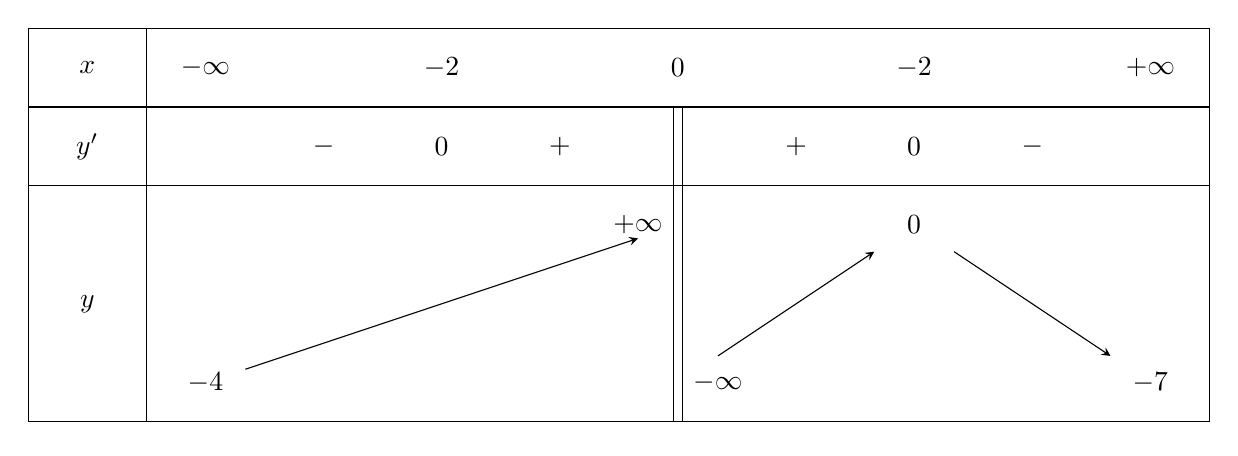
\begin{tikzpicture}[yscale=1,xscale=1.5]
            \def\c{9}%số cột
            \def\d{4}%số dòng
            \foreach \x in {0,...,\c}{
                \foreach \y in {0,...,\d}
                \path[yscale=-1] (\x,\y) node[gray!0,minimum size=1cm] (\x\y) {\x\y};
            }
            \path
            foreach \x/\t in {0/x,1/-\infty,3/-2,5/0,7/-2,9/+\infty} {(\x0) node {$\t$}}
            foreach \x/\t in {0/y',2/-,3/0,4/+,6/+,7/0,8/-} {(\x1) node {$\t$}}
            foreach \x/\t in {03/y,14/-4,52.west/+\infty,54.east/-\infty,72/0,94/-7} {(\x) node {$\t$}}
            ;
            \foreach \a/\b in {14/52,54/72,72/94} \draw[->,>=stealth] (\a)--(\b);
            \draw[double distance=3pt] (51.north)--(54.south);
            \draw[shift={(-0.5,0.5)}] (0,0) rectangle (\c+1,-\d-1)
            (0,-1)--(\c+1,-1) (0,-2)--(\c+1,-2) (1,0)--(1,-\d-1);
        \end{tikzpicture}
    \end{center}
    \choice
    {$-4 \leq m < 0$}
    {\True $-4 < m < 0$}
    {$-7 < m < 0$}
    {$-4 < m \leq 0$}
    \loigiai{ Để phương trình $f(x) = m$ có ba nghiệm phân biệt thì $-4 < m < 0$.
    }
\end{ex}
\begin{ex}%[2D1B5-3]
    Cho bảng biến thiên của hàm số $y = f(x)$. Tìm tất cả các giá trị của tham số $m$ để phương trình $f(x) = m$ có $3$ nghiệm phân biệt?
    \begin{center}
        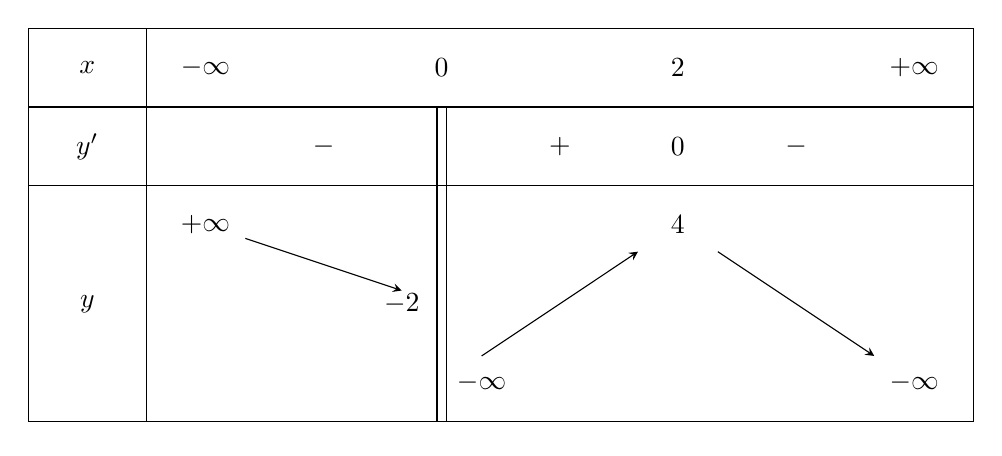
\begin{tikzpicture}[yscale=1,xscale=1.5]
            \def\c{7}%số cột
            \def\d{4}%số dòng
            \foreach \x in {0,...,\c}{
                \foreach \y in {0,...,\d}
                \path[yscale=-1] (\x,\y) node[gray!0,minimum size=1cm] (\x\y) {\x\y};
            }
            \path
            foreach \x/\t in {0/x,1/-\infty,3/0,5/2,7/+\infty} {(\x0) node {$\t$}}
            foreach \x/\t in {0/y',2/-,4/+,5/0,6/-} {(\x1) node {$\t$}}
            foreach \x/\t in {03/y,12/+\infty,33.west/-2,34.east/-\infty,52/4,74/-\infty} {(\x) node {$\t$}}
            ;
            \foreach \a/\b in {12/33,34/52,52/74} \draw[->,>=stealth] (\a)--(\b);
            \draw[double distance=3pt] (31.north)--(34.south);
            \draw[shift={(-0.5,0.5)}] (0,0) rectangle (\c+1,-\d-1)
            (0,-1)--(\c+1,-1) (0,-2)--(\c+1,-2) (1,0)--(1,-\d-1);
        \end{tikzpicture}
    \end{center}
    \choice
    {$m \in \left[ -2; 4\right]$}
    {\True $m \in \left( -2; 4\right)$}
    {$m \in \left( -2; 4\right]$}
    {$m \in \left( -\infty; 4\right]$}
    \loigiai{ Để phương trình $f(x) = m$ có ba nghiệm phân biệt thì $-2 < m < 4$.
    }
\end{ex}
\begin{ex}%[2D1K5-3]
    Cho hàm số $y = f(x)$ xác định trên $\left[0; +\infty\right)$ liên tục trên khoảng $(0; +\infty)$ và có bảng biến thiên như hình. Tìm tập hợp tất cả các giá trị thực của tham số $m$ sao cho phương trình $f(x) = m$ có hai
    nghiệm $x_1, x_2$ thỏa mãn $x_1 \in (0; 2)$ và $x_2 \in (2; +\infty)$.
    \begin{center}
        \begin{tikzpicture}[yscale=1,xscale=1.5]
            \def\c{8}%số cột
            \def\d{4}%số dòng
            \foreach \x in {0,...,\c}{
                \foreach \y in {0,...,\d}
                \path[yscale=-1] (\x,\y) node[gray!0,minimum size=1cm] (\x\y) {\x\y};
            }
            \fill[pattern=north east lines] ([xshift=-1.5mm]11.north west) rectangle (24.south);
            \path
            (24) node{$-2$}
            foreach \x/\t in {0/x,1/-\infty,2/0,4/1,6/2,8/+\infty} {(\x0) node {$\t$}}
            foreach \x/\t in {0/y',3/+,4/0,5/-,6/0,7/-} {(\x1) node {$\t$}}
            foreach \x/\t in {03/y,24/-2,42/0,63/-1,84/-3} {(\x) node {$\t$}}
            ;
            \foreach \a/\b in {24/42,42/63,63/84} \draw[->,>=stealth] (\a)--(\b);
            \draw[double distance=3pt] (21.north)--(22.north);
            \draw (22.north)--(24.south);
            \draw[shift={(-0.5,0.5)}] (0,0) rectangle (\c+1,-\d-1)
            (0,-1)--(\c+1,-1) (0,-2)--(\c+1,-2) (1,0)--(1,-\d-1);
        \end{tikzpicture}
    \end{center}
    \choice
    {\True $(-2; -1)$}
    {$\left[-2; -1\right)$}
    {$(-2; 0)$}
    {$(-3; -1)$}
    \loigiai{Theo giả thiết, phương trình $f(x) = m$ có hai nghiệm $x_1 \in (0; 2)$ và $x_2 \in (2; +\infty)$ khi đó
        $$\heva{& -2 < m \leq 0\\& -3 < m < -1} \Leftrightarrow -2 < m < -1.$$
    }
\end{ex}
\begin{ex}%[2D1K5-3]
    Cho bảng biến thiên của hàm số $y = f(x)$. Tìm $m$ để phương trình $f(x) - 1 = 2m$ có $3$ nghiệm
    phân biệt $x_1, x_2, x_3$ thỏa mãn $x_1 < 1 < x_2 < 2 < x_3$.
    \begin{center}
        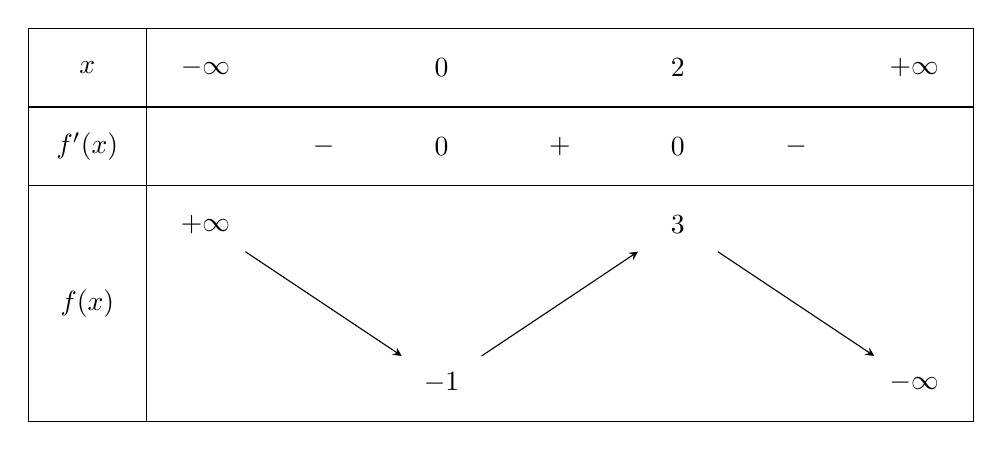
\begin{tikzpicture}[>=stealth,yscale=1,xscale=1.5]
            \def\c{7}%số cột
            \def\d{4}%số dòng
            \foreach \x in {0,...,\c}{
                \foreach \y in {0,...,-\d}
                \pgfmathsetmacro{\yy}{int(abs(\y))}
                \node[gray!0,minimum size=1cm] at (\x,\y) (\x\yy) {\x\yy};
            }
            \draw[shift={(-0.5,0.5)}]
            (0,0) rectangle (\c+1,-\d-1)
            (0,-1)--(\c+1,-1)
            (0,-2)--(\c+1,-2)
            (1,0)--(1,-\d-1);
            \path
            (00) node {$x$}
            (01) node {$f'(x)$}
            (03) node {$f(x)$}
            (10) node {$-\infty$}
            (30) node {$0$}
            (50) node {$2$}
            (70) node {$+\infty$}
            (21) node {$-$}
            (31) node {$0$}
            (41) node {$+$}
            (51) node {$0$}
            (61) node {$-$}
            (12) node {$+\infty$}
            (34) node {$-1$}
            (52) node {$3$}
            (74) node {$-\infty$};
            \draw[->] (12)--(34);
            \draw[->] (34)--(52);
            \draw[->] (52)--(74);
        \end{tikzpicture}
    \end{center}
    \choice
    {$-1 < m \leq 1$}
    {$-1 < m < 1$}
    {\True $0 < m < 1$}
    {$0 < m \leq 1$}
    \loigiai{Theo giả thiết, phương trình $f(x) = 2m + 1$ có ba nghiệm thỏa mãn hệ điều kiện
        \begin{eqnarray*}
            \heva{& x_1 < 1 \\& 1 < x_2 < 2\\& x_3 > 2} \Leftrightarrow \heva{& 2m + 1 \geq -1 \\& f(1) < 2m + 1 < 3 \\& 2m + 1 < 3 } \Leftrightarrow \heva{& m \geq -1 \\& \dfrac{f(1) - 1}{2} < m < 1 \\& m < 1 } \Leftrightarrow \dfrac{f(1) - 1}{2} < m < 1.
        \end{eqnarray*}
        Như vậy, ta cần phải xác định giá trị $f(1)$. Giả sử $f(x) = ax^3 + bx^2 + cx + d$. Khi đó $f'(x) = 3ax^2 + 2bx + c$. Từ bảng biến thiên, ta có hệ phương trình
        $$\heva{& f'(0) = 0\\& f'(2) = 0\\& f(0) = -1\\& f(2) = 3} \Leftrightarrow \heva{& c = 0\\& 12a + 4b = 0\\& d = -1 \\& 8a + 4b -1 = 0} \Leftrightarrow \heva{& a = - \dfrac{1}{4} \\& b = \dfrac{3}{4} \\& c = 0\\& d = -1}.$$
        Do đó $f(x) = -\dfrac{x^3}{4} + \dfrac{3}{4}x^2 - 1$. Từ đây ta có $f(1) = -\dfrac{1}{2}$. Vậy $-\dfrac{3}{4} < m < 1$.
    }
\end{ex}
\begin{ex}%[2D1K5-3]
    %câu 57
    (\textbf{Đề tham khảo thi THPT năm 2020 - Bộ GD \& ĐT}) Cho hàm số $=f(x)$ có bảng biến thiên như hình dưới. Số nghiệm thuộc đoạn $\left[ 0;\dfrac{5\pi}{2}\right] $của phương trình $f\left(\sin x\right) = 1$ là
    \begin{center}
        
\begin{tikzpicture}[>=stealth]
            \tkzTabInit[nocadre,lgt=1,espcl=2,deltacl=0.5]{$x$/.7 ,$y'$/.7,$y$/2}
            {$-\infty$ , $-1$ , $0$ , $1$ , $+\infty$}
            \tkzTabLine{ , + , $0$ , - , $0$ , + , $0$ , - , }
            \tkzTabVar{-/$-\infty$ , +/$2$, -/$0$ , +/$2$ , -/$-\infty$}
        \end{tikzpicture}
    \end{center}
    \choice
    {$4$}
    {$7$}
    {$6$}
    {\True $9$}
    \loigiai{
        Dựa vào bảng biến thiên của hàm số $f(x)$, ta có
        $$f\left(\sin x\right)=1 \Leftrightarrow \hoac{& \sin x=t_1 \in (- \infty;-1) &(1) \\ & \sin x=t_2 \in (-1;0) &(2)\\ & \sin x =t_3 \in (0;1) &(3) \\ & \sin x =t_4 \in (1;+\infty).&(4)} $$
        Đồ thị hàm số $y=\sin x$ trên đoạn $\left[0 ;\dfrac{5\pi}{2}\right]$
        \begin{center}
            \begin{tikzpicture}[line join = round, line cap = round,>=stealth,thick]
                %Vẽ hệ trục Oxy
                \draw[->,line width = 1pt] (-1,0)--(0,0) node[below right]{$O$}--(9,0) node[below]{$x$};
                \draw[->,line width = 1pt] (0,-1.5)--(0,1.5) node[left]{$y$};
                \fill (0,0) circle (1.5pt);
                %Vẽ đồ thị hàm số
                \draw[samples=300,domain=0:2.5*pi,smooth,blue!50!black] plot (\x, {sin(\x r)});
                %Vẽ các điểm trên hệ trục
                \foreach \x in {pi,2*pi,2.5*pi} \draw[thin] (\x,1pt)--(\x,-2pt);
                \foreach \y in {-1,1} \draw[thin] (1pt,\y)--(-1pt,\y) node [left] {$\y$};
                \node at (pi,0) [below] {$\pi$};
                \node at (2*pi,0) [below] {$2\pi$};
                \node at (2.5*pi,0) [below] {$\tfrac{5\pi}{2}$};
                \node[blue!50!black] at (2,1) [above] {$y = \sin x$};
                \draw [red]
                (-0.9,-0.7)--(8.9,-0.7)node[below right]{$ y=t_2 $}
                (-0.9,0.6)--(8.9,0.6)node[above right]{$ y=t_3 $};
                \draw[dashed](2.5*pi,0)--(2.5*pi,1);
            \end{tikzpicture}
        \end{center}
        Từ đồ thị trên ta suy ra
        \begin{itemize}
            \item Phương trình $(1)$ và phương trình $(4)$ vô nghiệm.
            \item Phương trình $(2)$ có $2$ nghiệm phân biệt.
            \item Phương trình $(3)$ có $3$ nghiệm phân biệt khác các nghiệm của phương trình $(2)$.
        \end{itemize}
        Vậy phương trình $f\left(\sin x\right)=1$ có $5$ nghiệm thuộc đoạn $\left[0 ;\dfrac{5\pi}{2}\right]$.
    }
\end{ex}
\begin{ex}%[2D1K5-3]
    Cho đồ thị hàm số $y = x^3 - 3x - 1$. Tìm $m$ để $\left|x^3 - 3x - 1\right|$ có $3$ nghiệm phân biệt.
    \begin{center}
        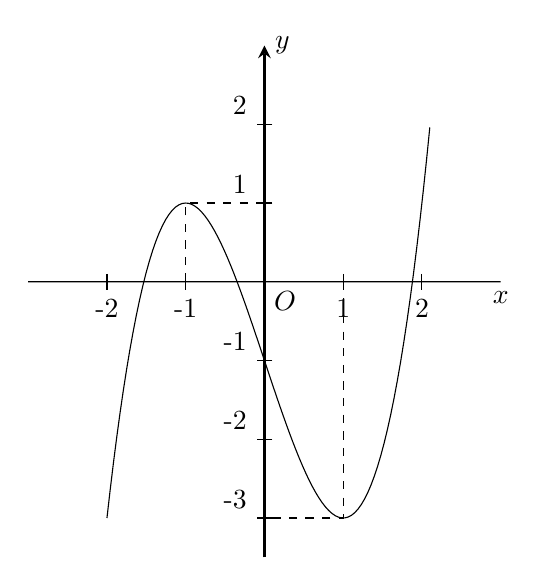
\begin{tikzpicture}[>=stealth]
            \draw[->] (-3,0)--(0,0) node[below right]{$O$}circle(.5pt)--(3,0) node[below]{$x$};
            \draw[->,line width = 1pt] (0,-3.5) --(0,3) node[right]{$y$};
            \foreach \x in {-2,-1,1,2}{\draw (\x,.1)--(\x,-.1)node[below]{\x};}
            \foreach \y in {-3,-2, -1, 1, 2}{\draw (.1,\y)--(-.1,\y)node[above left]{\y};
            }
            \draw [domain=-2:2.1, samples=100] %
            plot (\x, {(\x)^3-3*(\x)-1});
            \draw [dashed] (-1,0)--(-1,1)--(0,1);
            \draw [dashed] (1,0)--(1,-3)--(0,-3);
        \end{tikzpicture}
    \end{center}
    \choice
    {$m = 0$}
    {$1 < m < 3$}
    {$-3 < m < 1$}
    {\True $m = 0$ hoặc $m = 3$}
    \loigiai{ Từ đồ thị của hàm số $y = x^3 - 3x - 1$ ta có đồ thị của hàm số $y = \left| x^3 - 3x - 1\right|$ có dạng như hình bên dưới.
        \begin{center}
            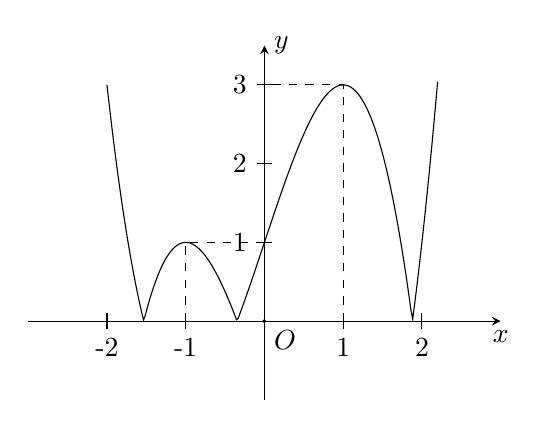
\begin{tikzpicture}[>=stealth]
                \draw[->] (-3,0) --(3,0)node[below]{$x$};% Trục Ok
                \draw[->] (0,-1) --(0,3.5) node[right]{$y$}; %Trục Ol
                \draw (0,0) node[below right]{$O$}circle(.5pt); %Điểm O
                \foreach \x in {-2,-1,1,2}{\draw (\x,.1)--(\x,-.1)node[below]{\x};
                }
                \foreach \y in {1,2,3}{\draw (.1,\y)--(-.1,\y)node[left]{\y};
                }
                \draw [domain=-2:2.2, samples=200] %
                plot (\x, {abs((\x)^3-3*(\x)-1)});
                \draw [dashed] (-1,0)--(-1,1)--(0,1);
                \draw [dashed] (1,0)--(1,3)--(0,3);
            \end{tikzpicture}
        \end{center}
        Từ đồ thị trên ta thấy rằng để phương trình $\left| x^3 - 3x - 1\right| = m$ có ba nghiệm phân biệt thì $m = 0$ hoặc $m = 3$.
    }
\end{ex}
\begin{ex}%[2D1K5-3]
    Cho đồ thị hàm số $y = f(x)$. Tìm tất cả các giá trị của tham số $m$ để phương trình $\left| f(x) \right| = m$ có
    $2$ nghiệm phân biệt?
    \begin{center}
        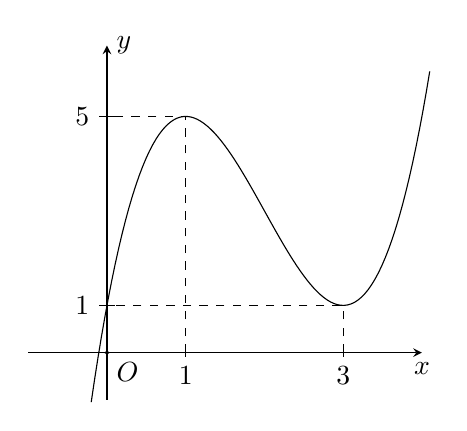
\begin{tikzpicture}[>=stealth, xscale = 1, yscale = .6]
            \draw[->] (-1,0) --(4,0)node[below]{$x$};% Trục Ok
            \draw[->] (0,-1) --(0,6.5) node[right]{$y$}; %Trục Ol
            \draw (0,0) node[below right]{$O$}circle(.7pt); %Điểm O
            \foreach \x in {1,3}{\draw (\x,.1)--(\x,-.1)node[below]{\x};}
            \foreach \y in {1, 5}{\draw (.1,\y)--(-.1,\y)node[left]{\y};
            }
            \draw [domain=-.2:4.1, samples=100] plot (\x, {(\x)^3 - 6*(\x)^2 + 9*(\x) + 1});
            \draw [dashed] (1,0)--(1,5)--(0,5);
            \draw [dashed] (3,0)--(3,1)--(0,1);
        \end{tikzpicture}
    \end{center}
    \choice
    {\True $\hoac{&0 < m < 1 \\& m > 5}$}
    {$m < 1$}
    {$m = 1, m = 5$}
    {$1 < m < 5$}
    \loigiai{Ta có đồ thị của hàm số $y = \left|f(x)\right|$ có dạng như hình bên dưới.
        \begin{center}
            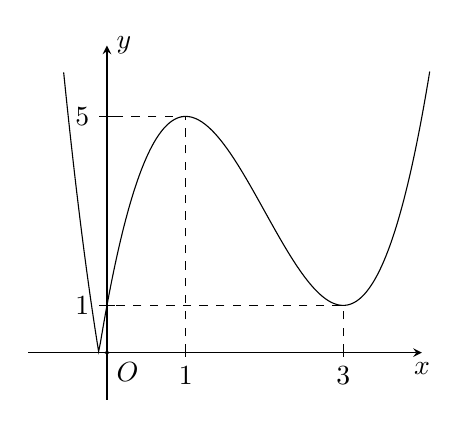
\begin{tikzpicture}[>=stealth, xscale = 1, yscale = .6]
                \draw[->] (-1,0) --(4,0)node[below]{$x$};% Trục Ok
                \draw[->] (0,-1) --(0,6.5) node[right]{$y$}; %Trục Ol
                \draw (0,0) node[below right]{$O$}circle(.7pt); %Điểm O
                \foreach \x in {1,3}{\draw (\x,.1)--(\x,-.1)node[below]{\x};}
                \foreach \y in {1, 5}{\draw (.1,\y)--(-.1,\y)node[left]{\y};
                }
                \draw [domain=-.55:4.1, samples=200] plot (\x, {abs((\x)^3 - 6*(\x)^2 + 9*(\x) + 1)});
                \draw [dashed] (1,0)--(1,5)--(0,5);
                \draw [dashed] (3,0)--(3,1)--(0,1);
            \end{tikzpicture}
        \end{center}
        Từ đồ thị trên ta thấy để phương trình $\left| f(x) \right| = m$ có $2$ nghiệm phân biệt khi $\hoac{& 0 < m < 1 \\& m > 5}$.
    }
\end{ex}
\begin{ex}%[2D1K5-3]
    Cho đồ thị hàm số $y = x^3 - 3x^2 + 2$ như hình vẽ. Tìm tất cả các giá trị của tham số $m$ để phương trình $\left| x \right|^3 - 3x^2 + 2 = m$ có nhiều nghiệm nhất?
    \begin{center}
        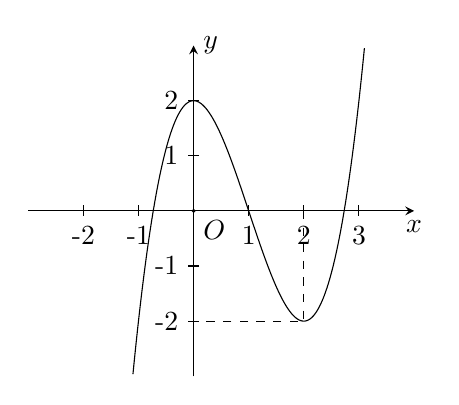
\begin{tikzpicture}[>=stealth, scale=0.7]
            \draw[->] (-3,0) --(4,0)node[below]{$x$};% Trục Ok
            \draw[->] (0,-3) --(0,3) node[right]{$y$}; %Trục Ol
            \draw (0,0) node[below right]{$O$}circle(.7pt); %Điểm O
            \foreach \x in {-2,-1,1,2,3}{\draw (\x,.1)--(\x,-.1)node[below]{\x};}
            \foreach \y in {-2,-1,1,2}{\draw (.1,\y)--(-.1,\y)node[left]{\y};
            }
            \draw [domain=-1.1:3.1, samples=150] plot (\x, {(\x)^3 - 3*(\x)^2 + 2});
            \draw [dashed] (2,0)--(2,-2)--(0,-2);
        \end{tikzpicture}
    \end{center}
    \choice
    {$-2 \leq m \leq 2$}
    {$0 < m < 2$}
    {\True $-2 < m < 2$}
    {$0 \leq m \leq 2$}
    \loigiai{Ta có đồ thị của hàm số $y = \left| x \right|^3 - 3x^2 + 2$ có dạng như hình bên dưới.
        \begin{center}
            \begin{tikzpicture}[>=stealth, xscale = 1, yscale = 1]
                \draw[->] (-4,0) --(4,0)node[below]{$x$};% Trục Ok
                \draw[->] (0,-3) --(0,3) node[right]{$y$}; %Trục Ol
                \draw (0,0) node[below right]{$O$}circle(.7pt); %Điểm O
                \foreach \x in {-2,-1,1,2,3}{\draw (\x,.1)--(\x,-.1)node[below]{\x};}
                \foreach \y in {-2,-1,1,2}{\draw (.1,\y)--(-.1,\y)node[left]{\y};
                }
                \draw [domain=-3.1:3.1, samples=150] plot (\x, {(abs(\x))^3 - 3*(\x)^2 + 2});
                \draw [dashed] (2,0)--(2,-2)--(0,-2)--(-2,-2)--(-2,0);
            \end{tikzpicture}
        \end{center}
        Do đó để phương trình $\left| x \right|^3 - 3x^2 + 2 = m$ có nhiều nghiệm nhất thì $-2 < m < 2$.
    }
\end{ex}
\begin{ex}%[2D1K5-3]
    Cho đồ thị hàm số $y = f(x)$ như hình vẽ. Tìm tất cả các giá trị của tham số $m$ để phương trình $f(\left| x \right|) = m$ có $2$ nghiệm phân biệt?
    \begin{center}
        \begin{tikzpicture}[>=stealth, xscale = 1, yscale = 1]
            \draw[->] (-2.5,0) --(3,0)node[below]{$x$};% Trục Ok
            \draw[->] (0,-1) --(0,3) node[right]{$y$}; %Trục Ol
            \draw (0,0) node[below right]{$O$}circle(.7pt); %Điểm O
            \foreach \x in {-1,1,2}{\draw (\x,.1)--(\x,-.1)node[below]{\x};}
            \foreach \y in {1,2}{\draw (.1,\y)--(-.1,\y)node[left]{\y};
            }
            \draw [domain=-.7:1.8, samples=100] plot (\x, {-2*(\x)^3 + 3*(\x)^2 + 1});
            \draw [dashed] (1,0)--(1,2)--(0,2);
        \end{tikzpicture}
    \end{center}
    \choice
    {$m \in (-\infty, 1) \cup (2, +\infty)$}
    {$m \in (-\infty, 1)$}
    {\True $m \in (-\infty, 1) \cup \left\lbrace 2\right\rbrace$}
    {$m \in (2, +\infty)$}
    \loigiai{Ta có đồ thị của hàm số $y = f(\left| x \right|)$ có dạng như hình bên dưới.
        \begin{center}
            \begin{tikzpicture}[>=stealth, xscale = 1, yscale = 1]
                \draw[->] (-3,0) --(3,0)node[below]{$x$};% Trục Ok
                \draw[->] (0,-1) --(0,3) node[right]{$y$}; %Trục Ol
                \draw (0,0) node[below right]{$O$}circle(.7pt); %Điểm O
                \foreach \x in {-2,-1,1,2}{\draw (\x,.1)--(\x,-.1)node[below]{\x};}
                \foreach \y in {1,2}{\draw (.1,\y)--(-.1,\y)node[below left]{\y};
                }
                \draw [domain=-1.8:1.8, samples=100] plot (\x, {-2*(abs(\x))^3 + 3*(\x)^2 + 1});
                \draw [dashed] (1,0)--(1,2)--(0,2)--(-1,2)--(-1,0);
            \end{tikzpicture}
        \end{center}
        Từ đồ thị trên ta thấy rằng để phương trình $f(\left| x \right|) = m$ có hai nghiệm phân biệt khi $m < 1$ hoặc $m = 2$.
    }
\end{ex}
\begin{ex}%[2D1K5-3]
    Cho bảng biến thiên của $y = f(x)$. Nếu $m \in (1, 3)$ thì $\left| f(x) \right| = m$ có bao nhiêu nghiệm?
    \begin{center}
        \begin{tikzpicture}[>=stealth,yscale=1,xscale=1.5]
            \def\c{7}%số cột
            \def\d{4}%số dòng
            \foreach \x in {0,...,\c}{
                \foreach \y in {0,...,-\d}
                \pgfmathsetmacro{\yy}{int(abs(\y))}
                \node[gray!0,minimum size=1cm] at (\x,\y) (\x\yy) {\x\yy};
            }
            \draw[shift={(-0.5,0.5)}]
            (0,0) rectangle (\c+1,-\d-1)
            (0,-1)--(\c+1,-1)
            (0,-2)--(\c+1,-2)
            (1,0)--(1,-\d-1);
            \path
            (00) node {$x$}
            (01) node {$f'(x)$}
            (03) node {$f(x)$}
            (10) node {$-\infty$}
            (30) node {$-1$}
            (50) node {$1$}
            (70) node {$+\infty$}
            (21) node {$-$}
            (31) node {$0$}
            (41) node {$+$}
            (51) node {$0$}
            (61) node {$-$}
            (12) node {$+\infty$}
            (34) node {$-4$}
            (52) node {$0$}
            (74) node {$-\infty$};
            \draw[->] (12)--(34);
            \draw[->] (34)--(52);
            \draw[->] (52)--(74);
        \end{tikzpicture}
    \end{center}
    \choice
    {\True $4$ nghiệm}
    {$3$ nghiệm}
    {$2$ nghiệm}
    {$5$ nghiệm}
    \loigiai{Đồ thị của hàm số $y = f(x)$ cắt trục $Ox$ tại $x = 0$ và $x = a$ (với $a < -1$ nào đó). Trên cơ sở đó, ta xây dựng bảng biến thiên của hàm số $y = \left| f(x) \right|$ có dạng
        \begin{center}
            \begin{tikzpicture}[>=stealth,yscale=1,xscale=1.5]
                \def\c{9}%số cột
                \def\d{4}%số dòng
                \foreach \x in {0,...,\c}{
                    \foreach \y in {0,...,-\d}
                    \pgfmathsetmacro{\yy}{int(abs(\y))}
                    \node[gray!0,minimum size=1cm] at (\x,\y) (\x\yy) {\x\yy};
                }
                \draw[shift={(-0.5,0.5)}]
                (0,0) rectangle (\c+1,-\d-1)
                (0,-1)--(\c+1,-1)
                (0,-2)--(\c+1,-2)
                (1,0)--(1,-\d-1);
                \path
                (00) node {$x$}
                (01) node {$y'$}
                (03) node {$y$}
                (10) node {$-\infty$}
                (30) node {$a$}
                (50) node {$-1$}
                (70) node {$1$}
                (90) node {$+\infty$}
                (21) node {$-$}
                (31) node {$0$}
                (41) node {$+$}
                (51) node {$0$}
                (61) node {$-$}
                (71) node {$0$}
                (81) node {$+$}
                (12) node {$+\infty$}
                (34) node {$0$}
                (52) node {$4$}
                (74) node {$0$}
                (92) node {$+\infty$};
                \draw[->] (12)--(34);
                \draw[->] (34)--(52);
                \draw[->] (52)--(74);
                \draw[->] (74)--(92);
            \end{tikzpicture}
        \end{center}
        Từ bảng biến thiên trên ta thấy với $m \in (1, 3)$ thì phương trình $\left| f(x) \right| = m$ có $4$ nghiệm phân biệt.
    }
\end{ex}

\Closesolutionfile{ans}